\documentclass[11pt,letterpaper]{article}

% =============================================================================
% PACKAGES
% =============================================================================
\usepackage[margin=1in]{geometry}
\usepackage{enumitem}
\usepackage{setspace}
\usepackage{graphicx}
\usepackage[table]{xcolor}
\usepackage{tikz}
\usetikzlibrary{shapes.geometric,shapes.symbols,arrows.meta,positioning,fit,backgrounds,calc,decorations.pathreplacing,trees,matrix,shapes.multipart,er}

% Default alignment for multi-line TikZ node labels
\tikzset{every node/.append style={align=center}}
\usepackage{tcolorbox}
\usepackage{booktabs}
\usepackage{longtable}
\usepackage{array}
\usepackage{tabularx}
\usepackage{multirow}
\usepackage{fancyhdr}
\usepackage{titlesec}
\usepackage[colorlinks=true,linkcolor=blue!60!black,urlcolor=blue!60!black,citecolor=blue!60!black]{hyperref}
\usepackage{bookmark}
\usepackage{parskip}
\usepackage{float}
\usepackage{caption}
\usepackage{subcaption}
\usepackage{listings}
\usepackage{microtype}
\usepackage{textcomp}
\usepackage{amssymb}

% =============================================================================
% CONFIGURATION
% =============================================================================
\setstretch{1.15}

% Define colors
\definecolor{primary}{RGB}{45, 80, 120}
\definecolor{secondary}{RGB}{70, 120, 150}
\definecolor{accent}{RGB}{180, 80, 50}
\definecolor{success}{RGB}{50, 130, 70}
\definecolor{lightgray}{RGB}{245, 245, 245}
\definecolor{darkgray}{RGB}{80, 80, 80}
\definecolor{entitycolor}{RGB}{220, 240, 255}
\definecolor{attributecolor}{RGB}{255, 250, 220}
\definecolor{relationcolor}{RGB}{230, 255, 230}
\definecolor{flowcolor}{RGB}{255, 235, 235}
\definecolor{storecolor}{RGB}{240, 230, 255}
\definecolor{processcolor}{RGB}{255, 245, 230}

% Section formatting
\titleformat{\section}{\Large\bfseries\color{primary}}{\thesection}{1em}{}[\titlerule]
\titleformat{\subsection}{\large\bfseries\color{secondary}}{\thesubsection}{1em}{}
\titleformat{\subsubsection}{\normalsize\bfseries\color{darkgray}}{\thesubsubsection}{1em}{}

% Header/Footer
\pagestyle{fancy}
\fancyhf{}
\fancyhead[L]{\small\textcolor{darkgray}{Information Viewpoint Specification}}
\fancyhead[R]{\small\textcolor{darkgray}{Architecture Documentation}}
\fancyfoot[C]{\thepage}
\renewcommand{\headrulewidth}{0.4pt}

% Custom environments
\newtcolorbox{definitionbox}[1][]{
    colback=lightgray,
    colframe=primary,
    fonttitle=\bfseries,
    title=#1,
    boxrule=0.5pt,
    arc=2pt,
    left=8pt,
    right=8pt,
    top=6pt,
    bottom=6pt
}

\newtcolorbox{examplebox}[1][]{
    colback=white,
    colframe=secondary,
    fonttitle=\bfseries,
    title=#1,
    boxrule=0.5pt,
    arc=2pt,
    left=8pt,
    right=8pt,
    top=6pt,
    bottom=6pt
}

\newtcolorbox{warningbox}[1][]{
    colback=orange!5,
    colframe=accent,
    fonttitle=\bfseries,
    title=#1,
    boxrule=0.5pt,
    arc=2pt,
    left=8pt,
    right=8pt,
    top=6pt,
    bottom=6pt
}

\newtcolorbox{guidancebox}[1][]{
    colback=green!5,
    colframe=success,
    fonttitle=\bfseries,
    title=#1,
    boxrule=0.5pt,
    arc=2pt,
    left=8pt,
    right=8pt,
    top=6pt,
    bottom=6pt
}

\newtcolorbox{patternbox}[1][]{
    colback=blue!3,
    colframe=primary!70,
    fonttitle=\bfseries,
    title=#1,
    boxrule=0.5pt,
    arc=2pt,
    left=8pt,
    right=8pt,
    top=6pt,
    bottom=6pt
}

\newtcolorbox{privacybox}[1][]{
    colback=purple!5,
    colframe=purple!70,
    fonttitle=\bfseries,
    title=#1,
    boxrule=0.5pt,
    arc=2pt,
    left=8pt,
    right=8pt,
    top=6pt,
    bottom=6pt
}

% Listings configuration
\lstset{
    basicstyle=\ttfamily\small,
    backgroundcolor=\color{lightgray},
    frame=single,
    framerule=0.5pt,
    rulecolor=\color{darkgray},
    breaklines=true,
    captionpos=b,
    tabsize=2,
    showstringspaces=false,
    numbers=left,
    numberstyle=\tiny\color{darkgray},
    numbersep=5pt,
    xleftmargin=15pt
}

\lstdefinelanguage{sql}{
    keywords={SELECT, FROM, WHERE, JOIN, ON, INSERT, UPDATE, DELETE, CREATE, TABLE, INDEX, PRIMARY, KEY, FOREIGN, REFERENCES, NOT, NULL, UNIQUE, DEFAULT, AND, OR, IN, AS, ORDER, BY, GROUP, HAVING, LIMIT, OFFSET, INNER, LEFT, RIGHT, OUTER, CASCADE, SET, VALUES, INTO, ALTER, DROP, CONSTRAINT, CHECK, BETWEEN, LIKE, EXISTS, UNION, ALL, DISTINCT, CASE, WHEN, THEN, ELSE, END},
    sensitive=false,
    comment=[l]{--},
    morecomment=[s]{/*}{*/},
    morestring=[b]',
    morestring=[b]"
}

% Table column types
\newcolumntype{L}[1]{>{\raggedright\arraybackslash}p{#1}}
\newcolumntype{C}[1]{>{\centering\arraybackslash}p{#1}}
\newcolumntype{R}[1]{>{\raggedleft\arraybackslash}p{#1}}

% =============================================================================
% DOCUMENT BEGIN
% =============================================================================
\begin{document}

% -----------------------------------------------------------------------------
% TITLE PAGE
% -----------------------------------------------------------------------------
\hypersetup{pageanchor=false}
\begin{titlepage}
    \centering
    \vspace*{1.5cm}
    
    {\Huge\bfseries\color{primary} Information Viewpoint\par}
    \vspace{0.5cm}
    {\Large\color{secondary} Architecture Viewpoint Specification\par}
    \vspace{0.3cm}
    {\large\color{darkgray} Data Architecture \& Information Management\par}
    
    \vspace{1.3cm}
    
    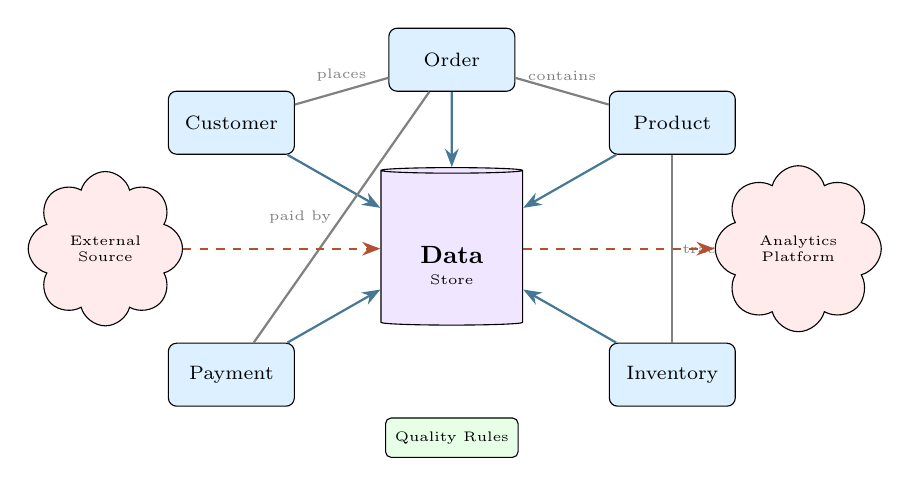
\begin{tikzpicture}[scale=0.8]
        % Central data store
        \node[draw, cylinder, shape border rotate=90, aspect=0.3, minimum height=2cm, minimum width=1.8cm, fill=storecolor] (db) at (0,0) {};
        \node[font=\small\bfseries] at (0, -0.1) {Data};
        \node[font=\tiny] at (0, -0.5) {Store};
        
        % Entity boxes around
        \node[draw, fill=entitycolor, rounded corners=3pt, minimum width=1.6cm, minimum height=0.8cm, font=\scriptsize] (e1) at (-3.5, 2) {Customer};
        \node[draw, fill=entitycolor, rounded corners=3pt, minimum width=1.6cm, minimum height=0.8cm, font=\scriptsize] (e2) at (0, 3) {Order};
        \node[draw, fill=entitycolor, rounded corners=3pt, minimum width=1.6cm, minimum height=0.8cm, font=\scriptsize] (e3) at (3.5, 2) {Product};
        \node[draw, fill=entitycolor, rounded corners=3pt, minimum width=1.6cm, minimum height=0.8cm, font=\scriptsize] (e4) at (-3.5, -2) {Payment};
        \node[draw, fill=entitycolor, rounded corners=3pt, minimum width=1.6cm, minimum height=0.8cm, font=\scriptsize] (e5) at (3.5, -2) {Inventory};
        
        % Data flows
        \draw[-{Stealth}, thick, secondary] (e1) -- (db);
        \draw[-{Stealth}, thick, secondary] (e2) -- (db);
        \draw[-{Stealth}, thick, secondary] (e3) -- (db);
        \draw[-{Stealth}, thick, secondary] (e4) -- (db);
        \draw[-{Stealth}, thick, secondary] (e5) -- (db);
        
        % Relationships
        \draw[thick, gray] (e1) -- (e2) node[midway, above, font=\tiny] {places};
        \draw[thick, gray] (e2) -- (e3) node[midway, above, font=\tiny] {contains};
        \draw[thick, gray] (e2) -- (e4) node[midway, left, font=\tiny] {paid by};
        \draw[thick, gray] (e3) -- (e5) node[midway, right, font=\tiny] {tracked in};
        
        % External sources
        \node[draw, cloud, cloud puffs=8, fill=flowcolor, minimum width=1.5cm, minimum height=0.8cm, font=\tiny] (ext1) at (-5.5, 0) {External\\Source};
        \node[draw, cloud, cloud puffs=8, fill=flowcolor, minimum width=1.5cm, minimum height=0.8cm, font=\tiny] (ext2) at (5.5, 0) {Analytics\\Platform};
        
        \draw[-{Stealth}, thick, dashed, accent] (ext1) -- (db);
        \draw[-{Stealth}, thick, dashed, accent] (db) -- (ext2);
        
        % Data quality indicator
        \node[draw, fill=relationcolor, rounded corners=2pt, minimum width=1.2cm, minimum height=0.5cm, font=\tiny] at (0, -3) {Quality Rules};
    \end{tikzpicture}
    
    \vspace{1.5cm}
    
    \begin{tabular}{ll}
        \textbf{Version:} & 2.0 \\
        \textbf{Status:} & Release \\
        \textbf{Classification:} & ISO/IEC/IEEE 42010 Compliant \\
        \textbf{Last Updated:} & \today \\
    \end{tabular}
    
    \vfill
    
    {\small Based on the Views and Beyond approach to software architecture documentation}
    
\end{titlepage}
\clearpage
\hypersetup{pageanchor=true}

% -----------------------------------------------------------------------------
% TABLE OF CONTENTS
% -----------------------------------------------------------------------------
\tableofcontents
\newpage

% =============================================================================
% SECTION: VIEWPOINT NAME
% =============================================================================
\section{Viewpoint Name}

\begin{definitionbox}[Viewpoint Identification]
\begin{tabular}{@{}L{3.5cm}L{10cm}@{}}
\textbf{Name:} & Information Viewpoint \\[0.5em]
\textbf{Synonyms:} & Data Viewpoint, Data Architecture View, Information Architecture View, Data Model View, Conceptual Data View, Logical Data View, Data Flow View \\[0.5em]
\textbf{Identifier:} & VP-INFO-001 \\[0.5em]
\textbf{Version:} & 2.0 \\
\end{tabular}
\end{definitionbox}

\subsection{Viewpoint Classification}

The Information Viewpoint addresses data-centric concerns within software architecture. While not explicitly defined as a single style in the original Views and Beyond approach, it represents a critical cross-cutting concern that intersects with module, component-and-connector, and allocation viewpoints. This viewpoint provides a unified perspective on how data is structured, stored, flows through, and is managed by the system.

\begin{table}[H]
\centering
\caption{Viewpoint Classification Taxonomy}
\begin{tabular}{@{}L{4cm}L{10cm}@{}}
\toprule
\textbf{Attribute} & \textbf{Value} \\
\midrule
Style Family & Cross-Cutting / Data-Centric \\
Primary Focus & Data Structure, Flow, Storage, and Governance \\
Abstraction Level & Conceptual, Logical, and Physical \\
Temporal Perspective & Static Structure and Dynamic Flow \\
Related Styles & Data Model, Data Flow, Repository \\
IEEE 42010 Category & Information Viewpoint \\
TOGAF Equivalent & Data Architecture \\
\bottomrule
\end{tabular}
\end{table}

\subsection{Viewpoint Scope}

The Information Viewpoint encompasses multiple perspectives on data within a system:

\begin{itemize}
    \item \textbf{Conceptual Data Model:} Business-oriented view of data entities and relationships independent of implementation, expressed in terms familiar to business stakeholders.
    
    \item \textbf{Logical Data Model:} Detailed structure of data entities, attributes, relationships, and constraints without physical implementation details.
    
    \item \textbf{Physical Data Model:} Implementation-specific data structures including tables, columns, indexes, partitions, and storage configurations.
    
    \item \textbf{Data Flow Model:} Movement of data through system components, transformations applied, and integration patterns used.
    
    \item \textbf{Data Lifecycle Model:} States data passes through from creation to archival or deletion, including retention policies.
    
    \item \textbf{Data Quality Model:} Rules, constraints, and processes ensuring data accuracy, completeness, and consistency.
    
    \item \textbf{Data Security Model:} Classification, access control, encryption, and privacy protection mechanisms.
\end{itemize}

% =============================================================================
% SECTION: OVERVIEW
% =============================================================================
\section{Overview}

The Information Viewpoint provides a comprehensive framework for documenting the data architecture of a software system. It addresses how data is structured, stored, accessed, transformed, and governed throughout its lifecycle. In modern data-driven systems, this viewpoint is essential for ensuring data quality, consistency, security, and compliance.

\subsection{Purpose and Scope}

The primary purpose of this viewpoint is to establish a clear understanding of the system's data assets, their structures and relationships, where data resides, how it flows between components, and how it is protected and governed. This understanding is critical for system design, integration, compliance, and evolution.

\begin{definitionbox}[Viewpoint Definition]
The Information Viewpoint defines the structure, semantics, storage, flow, and governance of data within a system. It encompasses data entities and their relationships, data storage mechanisms, data movement patterns, data quality rules, and data protection measures. This viewpoint bridges business information needs with technical data implementation.
\end{definitionbox}

\subsection{Key Characteristics}

The Information Viewpoint exhibits several distinctive characteristics:

\textbf{Multi-Level Abstraction:} Data architecture is documented at conceptual (business), logical (design), and physical (implementation) levels, enabling communication with different stakeholder groups and supporting design refinement.

\textbf{Static and Dynamic Perspectives:} The viewpoint captures both static data structures (entities, relationships, schemas) and dynamic data behavior (flows, transformations, lifecycle states).

\textbf{Cross-System Scope:} Data often spans multiple systems, databases, and services. This viewpoint addresses data integration, synchronization, and consistency across system boundaries.

\textbf{Governance Integration:} Data governance concerns including quality, security, privacy, and compliance are integral to this viewpoint, not afterthoughts.

\textbf{Business Alignment:} Data models explicitly connect to business concepts, ensuring that technical data structures support business information requirements.

\subsection{Relationship to Other Viewpoints}

The Information Viewpoint connects to other architectural viewpoints in significant ways:

\begin{table}[H]
\centering
\caption{Relationships to Other Viewpoints}
\begin{tabular}{@{}L{3.5cm}L{10.5cm}@{}}
\toprule
\textbf{Viewpoint} & \textbf{Relationship} \\
\midrule
Development & Data model entities are implemented as domain classes/modules. Repository patterns connect data to code. \\
\addlinespace
Component-and-Connector & Data stores are components; data flows are connectors. Runtime data access patterns are defined. \\
\addlinespace
Deployment & Physical data stores are deployed to infrastructure. Replication and distribution strategies are realized. \\
\addlinespace
Security & Data classification drives security controls. Access policies map to data elements. Encryption requirements apply. \\
\addlinespace
Operational & Backup, recovery, and archival procedures apply to data stores. Monitoring covers data health. \\
\addlinespace
Business/Functional & Business entities map to data entities. Business rules become data constraints. \\
\bottomrule
\end{tabular}
\end{table}

\subsection{Data Architecture Layers}

\begin{figure}[H]
\centering
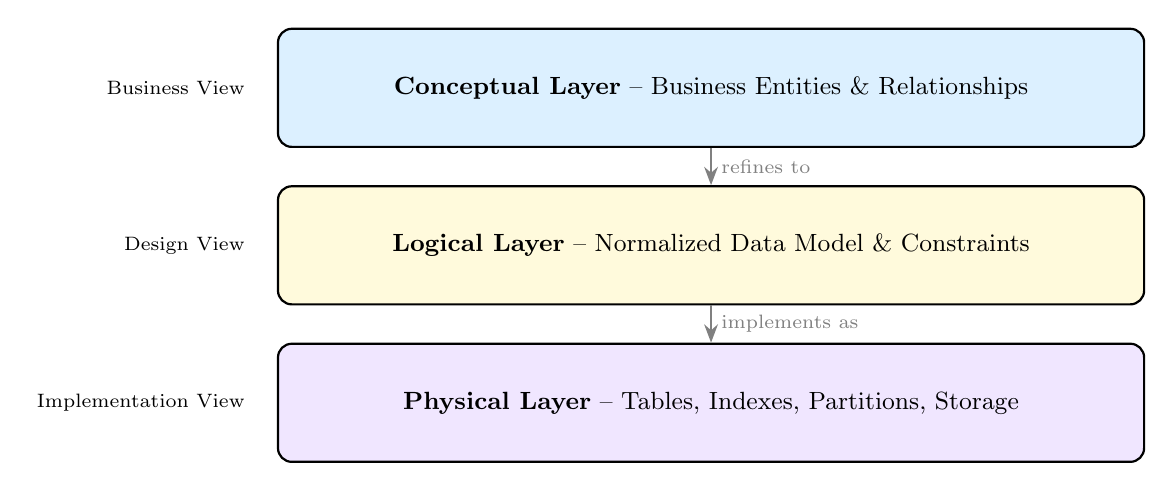
\begin{tikzpicture}[
    node distance=1.2cm,
    layer/.style={draw, thick, rounded corners=5pt, minimum width=11cm, minimum height=1.5cm, font=\small},
    arrow/.style={-{Stealth}, thick, gray}
]
    % Layers
    \node[layer, fill=entitycolor] (concept) at (0, 4.5) {\textbf{Conceptual Layer} -- Business Entities \& Relationships};
    \node[layer, fill=attributecolor] (logical) at (0, 2.5) {\textbf{Logical Layer} -- Normalized Data Model \& Constraints};
    \node[layer, fill=storecolor] (physical) at (0, 0.5) {\textbf{Physical Layer} -- Tables, Indexes, Partitions, Storage};
    
    % Arrows
    \draw[arrow] (concept) -- (logical) node[midway, right, font=\scriptsize] {refines to};
    \draw[arrow] (logical) -- (physical) node[midway, right, font=\scriptsize] {implements as};
    
    % Side labels
    \node[font=\scriptsize, anchor=east] at (-5.8, 4.5) {Business View};
    \node[font=\scriptsize, anchor=east] at (-5.8, 2.5) {Design View};
    \node[font=\scriptsize, anchor=east] at (-5.8, 0.5) {Implementation View};
    
\end{tikzpicture}
\caption{Data Architecture Abstraction Layers}
\end{figure}

% =============================================================================
% SECTION: CONCERNS
% =============================================================================
\section{Concerns}

This section enumerates the architectural concerns that the Information Viewpoint is designed to address. These concerns represent the fundamental questions stakeholders have about the system's data architecture.

\subsection{Primary Concerns}

\begin{enumerate}[label=\textbf{C\arabic*:}, leftmargin=2.5em]
    \item \textbf{Data Structure and Modeling}
    \begin{itemize}[nosep]
        \item What are the key data entities in the system?
        \item What attributes define each entity?
        \item What relationships exist between entities?
        \item What constraints ensure data integrity?
        \item How does the data model align with business concepts?
    \end{itemize}
    
    \item \textbf{Data Storage and Persistence}
    \begin{itemize}[nosep]
        \item Where is data physically stored?
        \item What database technologies are used?
        \item How is data partitioned and distributed?
        \item What indexing strategies optimize access?
        \item How is storage capacity planned and managed?
    \end{itemize}
    
    \item \textbf{Data Flow and Integration}
    \begin{itemize}[nosep]
        \item How does data move through the system?
        \item What transformations are applied to data?
        \item How is data synchronized across systems?
        \item What integration patterns are used (ETL, CDC, API)?
        \item How is data consistency maintained across boundaries?
    \end{itemize}
    
    \item \textbf{Data Quality and Integrity}
    \begin{itemize}[nosep]
        \item What rules ensure data accuracy?
        \item How is data completeness validated?
        \item What processes detect and correct data errors?
        \item How is data freshness maintained?
        \item What metrics measure data quality?
    \end{itemize}
    
    \item \textbf{Data Security and Privacy}
    \begin{itemize}[nosep]
        \item How is sensitive data classified?
        \item What access controls protect data?
        \item How is data encrypted at rest and in transit?
        \item What data masking or anonymization is applied?
        \item How are privacy regulations (GDPR, CCPA) addressed?
    \end{itemize}
    
    \item \textbf{Data Lifecycle Management}
    \begin{itemize}[nosep]
        \item What states does data pass through?
        \item What retention policies apply?
        \item How is data archived?
        \item When and how is data deleted?
        \item How are lifecycle transitions triggered?
    \end{itemize}
    
    \item \textbf{Data Governance and Ownership}
    \begin{itemize}[nosep]
        \item Who owns each data domain?
        \item What stewardship responsibilities exist?
        \item How are data standards enforced?
        \item What approval processes govern data changes?
        \item How is data lineage tracked?
    \end{itemize}
    
    \item \textbf{Data Performance and Scalability}
    \begin{itemize}[nosep]
        \item What are data volume projections?
        \item How does the system handle data growth?
        \item What query performance requirements exist?
        \item How is data access optimized?
        \item What caching strategies are employed?
    \end{itemize}
    
    \item \textbf{Data Availability and Recovery}
    \begin{itemize}[nosep]
        \item What data redundancy exists?
        \item How is data backed up?
        \item What recovery point objectives (RPO) apply?
        \item What recovery time objectives (RTO) apply?
        \item How is data disaster recovery handled?
    \end{itemize}
    
    \item \textbf{Data Compliance and Audit}
    \begin{itemize}[nosep]
        \item What regulatory requirements affect data?
        \item How is data access audited?
        \item What compliance certifications are required?
        \item How is data sovereignty addressed?
        \item What audit trails are maintained?
    \end{itemize}
\end{enumerate}

\subsection{Concern-Quality Attribute Mapping}

\begin{table}[H]
\centering
\caption{Concern to Quality Attribute Mapping}
\small
\begin{tabular}{@{}L{3.2cm}C{1cm}C{1cm}C{1cm}C{1cm}C{1cm}C{1cm}C{1cm}C{1cm}@{}}
\toprule
\textbf{Concern} & \rotatebox{60}{\textbf{Integrity}} & \rotatebox{60}{\textbf{Security}} & \rotatebox{60}{\textbf{Performance}} & \rotatebox{60}{\textbf{Availability}} & \rotatebox{60}{\textbf{Scalability}} & \rotatebox{60}{\textbf{Compliance}} & \rotatebox{60}{\textbf{Maintaintic.}} & \rotatebox{60}{\textbf{Interop.}} \\
\midrule
Data Structure & $\bullet$ & $\circ$ & $\circ$ & -- & $\circ$ & $\circ$ & $\bullet$ & $\circ$ \\
Storage & $\circ$ & $\circ$ & $\bullet$ & $\bullet$ & $\bullet$ & $\circ$ & $\circ$ & -- \\
Flow/Integration & $\bullet$ & $\circ$ & $\circ$ & $\circ$ & $\circ$ & $\circ$ & $\circ$ & $\bullet$ \\
Quality & $\bullet$ & -- & -- & -- & -- & $\bullet$ & $\circ$ & $\circ$ \\
Security/Privacy & $\circ$ & $\bullet$ & $\circ$ & -- & -- & $\bullet$ & $\circ$ & -- \\
Lifecycle & $\circ$ & $\circ$ & $\circ$ & $\circ$ & $\bullet$ & $\bullet$ & $\bullet$ & -- \\
Governance & $\bullet$ & $\circ$ & -- & -- & -- & $\bullet$ & $\bullet$ & $\circ$ \\
Performance & -- & -- & $\bullet$ & $\circ$ & $\bullet$ & -- & $\circ$ & -- \\
Availability & $\circ$ & -- & $\circ$ & $\bullet$ & $\circ$ & $\circ$ & $\circ$ & -- \\
Compliance & $\circ$ & $\bullet$ & -- & $\circ$ & -- & $\bullet$ & $\circ$ & $\circ$ \\
\bottomrule
\multicolumn{9}{l}{\footnotesize $\bullet$ = Primary impact, $\circ$ = Secondary impact, -- = Minimal impact}
\end{tabular}
\end{table}

% =============================================================================
% SECTION: ANTI-CONCERNS
% =============================================================================
\section{Anti-Concerns}

Understanding what the Information Viewpoint is \emph{not} appropriate for helps stakeholders avoid misapplying this viewpoint.

\subsection{Out of Scope Topics}

\begin{enumerate}[label=\textbf{AC\arabic*:}, leftmargin=2.5em]
    \item \textbf{Application Logic and Behavior}
    \begin{itemize}[nosep]
        \item Business process workflows and orchestration
        \item Algorithm implementations and computation logic
        \item User interface behavior and interactions
        \item Service orchestration patterns
        \item Event-driven behavior specifications
    \end{itemize}
    
    \item \textbf{Infrastructure Details}
    \begin{itemize}[nosep]
        \item Server hardware specifications
        \item Network topology and routing
        \item Container orchestration configuration
        \item Operating system configuration
        \item Cloud infrastructure provisioning
    \end{itemize}
    
    \item \textbf{Code Organization}
    \begin{itemize}[nosep]
        \item Module decomposition and dependencies
        \item Class hierarchies and inheritance
        \item Package structure and namespaces
        \item Build system configuration
        \item Source code repository organization
    \end{itemize}
    
    \item \textbf{User Experience}
    \begin{itemize}[nosep]
        \item Screen designs and layouts
        \item Navigation flows
        \item Accessibility requirements
        \item Localization and internationalization UI
        \item User feedback and error messaging
    \end{itemize}
    
    \item \textbf{Project Management}
    \begin{itemize}[nosep]
        \item Development schedules and milestones
        \item Resource allocation and budgeting
        \item Risk management processes
        \item Team organization and roles
        \item Vendor management
    \end{itemize}
\end{enumerate}

\begin{warningbox}[Common Misapplications]
Avoid using the Information Viewpoint for:

\begin{itemize}[nosep]
    \item Documenting runtime component interactions (use C\&C Viewpoint)
    \item Specifying deployment topology (use Deployment Viewpoint)
    \item Defining code module structure (use Development Viewpoint)
    \item Detailing business processes (use Process/Functional Viewpoint)
    \item Specifying API contracts (use Interface Specifications)
\end{itemize}
\end{warningbox}

% =============================================================================
% SECTION: TYPICAL STAKEHOLDERS
% =============================================================================
\section{Typical Stakeholders}

The Information Viewpoint serves multiple stakeholder communities, each with distinct information needs about the system's data architecture.

\subsection{Primary Stakeholders}

\begin{table}[H]
\centering
\caption{Primary Stakeholder Analysis}
\small
\begin{tabular}{@{}L{2.6cm}L{3.6cm}L{7cm}@{}}
\toprule
\textbf{Stakeholder} & \textbf{Role Description} & \textbf{Primary Interests} \\
\midrule
Data Architects & Design enterprise data structures & Data modeling, naming standards, integration patterns, master data management \\
\addlinespace
Database Administrators & Manage database systems & Physical schemas, indexes, performance tuning, backup/recovery, storage management \\
\addlinespace
Data Engineers & Build data pipelines & ETL/ELT processes, data transformations, data quality, pipeline orchestration \\
\addlinespace
Data Stewards & Govern data domains & Data quality rules, business definitions, data ownership, compliance \\
\addlinespace
Privacy Officers & Ensure data privacy & Personal data inventory, consent management, privacy impact, regulatory compliance \\
\addlinespace
Security Architects & Protect data assets & Data classification, access control, encryption, threat modeling \\
\bottomrule
\end{tabular}
\end{table}

\subsection{Secondary Stakeholders}

\begin{table}[H]
\centering
\caption{Secondary Stakeholder Analysis}
\small
\begin{tabular}{@{}L{2.6cm}L{3.6cm}L{7cm}@{}}
\toprule
\textbf{Stakeholder} & \textbf{Role Description} & \textbf{Primary Interests} \\
\midrule
Software Developers & Implement applications & Domain models, data access APIs, ORM mappings, data validation \\
\addlinespace
Business Analysts & Define requirements & Business entities, data requirements, reporting needs, data dictionaries \\
\addlinespace
Data Scientists & Analyze data & Data availability, data quality, feature engineering, data access \\
\addlinespace
Compliance Officers & Ensure regulatory compliance & Audit trails, retention policies, data sovereignty, regulatory mapping \\
\addlinespace
Operations Teams & Maintain production systems & Data monitoring, incident response, capacity management, disaster recovery \\
\addlinespace
Business Stakeholders & Use data for decisions & Data definitions, data availability, reporting capabilities, data accuracy \\
\bottomrule
\end{tabular}
\end{table}

\subsection{Stakeholder Concern Matrix}

\begin{table}[H]
\centering
\caption{Stakeholder-Concern Responsibility Matrix}
\footnotesize
\begin{tabular}{@{}L{2.2cm}C{0.8cm}C{0.8cm}C{0.8cm}C{0.8cm}C{0.8cm}C{0.8cm}C{0.8cm}C{0.8cm}C{0.8cm}C{0.8cm}@{}}
\toprule
& \rotatebox{60}{\textbf{Structure}} & \rotatebox{60}{\textbf{Storage}} & \rotatebox{60}{\textbf{Flow}} & \rotatebox{60}{\textbf{Quality}} & \rotatebox{60}{\textbf{Security}} & \rotatebox{60}{\textbf{Lifecycle}} & \rotatebox{60}{\textbf{Governance}} & \rotatebox{60}{\textbf{Perform.}} & \rotatebox{60}{\textbf{Avail.}} & \rotatebox{60}{\textbf{Compliance}} \\
\midrule
Data Architect & R & A & R & A & C & A & R & C & C & C \\
DBA & C & R & C & C & A & C & I & R & R & I \\
Data Engineer & C & C & R & R & C & C & I & A & C & I \\
Data Steward & A & I & I & R & I & R & R & I & I & A \\
Privacy Officer & I & I & C & C & A & A & A & I & I & R \\
Security Arch. & C & C & C & I & R & C & C & I & C & A \\
\bottomrule
\multicolumn{11}{l}{\footnotesize R = Responsible, A = Accountable, C = Consulted, I = Informed}
\end{tabular}
\end{table}

% =============================================================================
% SECTION: MODEL TYPES
% =============================================================================
\section{Model Types}

The Information Viewpoint employs several complementary model types to capture different aspects of the data architecture. Each model type serves specific documentation purposes.

\subsection{Model Type Catalog}

\begin{enumerate}[label=\textbf{MT\arabic*:}, leftmargin=2.5em]
    \item \textbf{Conceptual Data Model}
    \begin{itemize}[nosep]
        \item \textit{Purpose:} Show business entities and relationships at high level
        \item \textit{Primary Elements:} Business entities, relationships, business rules
        \item \textit{Key Relationships:} Associates, contains, specializes
        \item \textit{Typical Notation:} Simplified ER diagram, concept maps
    \end{itemize}
    
    \item \textbf{Logical Data Model}
    \begin{itemize}[nosep]
        \item \textit{Purpose:} Define normalized data structures with full detail
        \item \textit{Primary Elements:} Entities, attributes, keys, relationships, constraints
        \item \textit{Key Relationships:} One-to-one, one-to-many, many-to-many
        \item \textit{Typical Notation:} ER diagrams (Chen, Crow's foot, IDEF1X)
    \end{itemize}
    
    \item \textbf{Physical Data Model}
    \begin{itemize}[nosep]
        \item \textit{Purpose:} Document implementation-specific database structures
        \item \textit{Primary Elements:} Tables, columns, indexes, partitions, constraints
        \item \textit{Key Relationships:} Foreign keys, triggers, procedures
        \item \textit{Typical Notation:} Database diagrams, DDL scripts
    \end{itemize}
    
    \item \textbf{Data Flow Diagram}
    \begin{itemize}[nosep]
        \item \textit{Purpose:} Show movement and transformation of data
        \item \textit{Primary Elements:} Processes, data stores, external entities, flows
        \item \textit{Key Relationships:} Data flow, transformation, aggregation
        \item \textit{Typical Notation:} DFD (Yourdon, Gane-Sarson), data pipelines
    \end{itemize}
    
    \item \textbf{Data Lineage Diagram}
    \begin{itemize}[nosep]
        \item \textit{Purpose:} Track data origin, transformations, and destinations
        \item \textit{Primary Elements:} Sources, transformations, targets, dependencies
        \item \textit{Key Relationships:} Derived-from, transformed-by, feeds-into
        \item \textit{Typical Notation:} Lineage graphs, dependency trees
    \end{itemize}
    
    \item \textbf{Data Classification Schema}
    \begin{itemize}[nosep]
        \item \textit{Purpose:} Document data sensitivity and handling requirements
        \item \textit{Primary Elements:} Classification levels, data categories, handling rules
        \item \textit{Key Relationships:} Classified-as, requires, governed-by
        \item \textit{Typical Notation:} Classification matrices, data catalogs
    \end{itemize}
    
    \item \textbf{Data Lifecycle Model}
    \begin{itemize}[nosep]
        \item \textit{Purpose:} Define states and transitions in data lifecycle
        \item \textit{Primary Elements:} States, transitions, triggers, retention periods
        \item \textit{Key Relationships:} Transitions-to, triggered-by, expires-after
        \item \textit{Typical Notation:} State diagrams, lifecycle charts
    \end{itemize}
    
    \item \textbf{Data Quality Rules Model}
    \begin{itemize}[nosep]
        \item \textit{Purpose:} Specify data quality constraints and validation rules
        \item \textit{Primary Elements:} Rules, dimensions, thresholds, remediation
        \item \textit{Key Relationships:} Validates, measures, triggers
        \item \textit{Typical Notation:} Rule tables, quality dashboards
    \end{itemize}
    
    \item \textbf{Master Data Model}
    \begin{itemize}[nosep]
        \item \textit{Purpose:} Define authoritative sources for shared data
        \item \textit{Primary Elements:} Master entities, golden records, sources
        \item \textit{Key Relationships:} Mastered-by, synchronized-from, authoritative-for
        \item \textit{Typical Notation:} MDM architecture diagrams
    \end{itemize}
\end{enumerate}

\subsection{Model Type Relationships}

\begin{figure}[H]
\centering
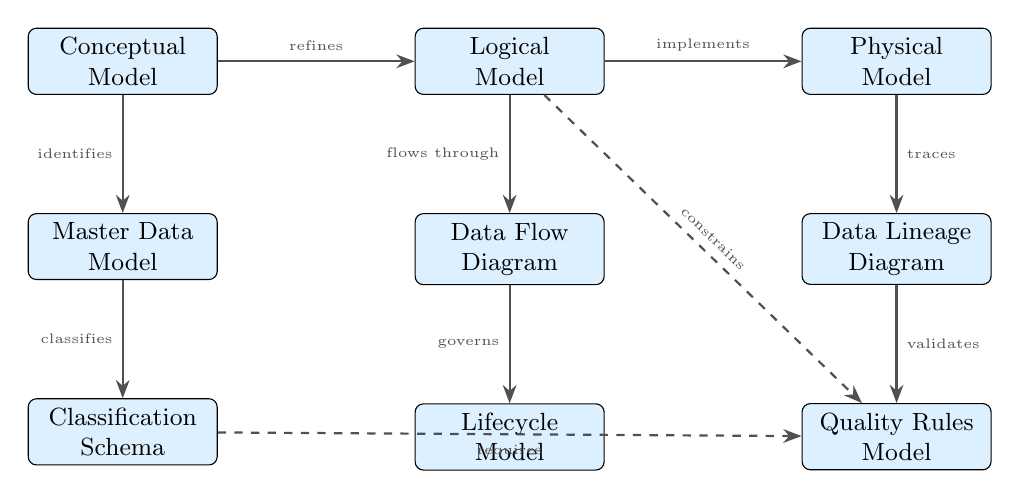
\begin{tikzpicture}[
    node distance=1.3cm and 2cm,
    model/.style={draw, fill=entitycolor, rounded corners=3pt, minimum width=2.4cm, minimum height=0.8cm, font=\small, align=center},
    arrow/.style={-{Stealth}, thick, darkgray}
]
    % Nodes - top row
    \node[model] (concept) {Conceptual\\Model};
    \node[model, right=2.5cm of concept] (logical) {Logical\\Model};
    \node[model, right=2.5cm of logical] (physical) {Physical\\Model};
    
    % Nodes - middle row
    \node[model, below=1.5cm of concept] (master) {Master Data\\Model};
    \node[model, below=1.5cm of logical] (flow) {Data Flow\\Diagram};
    \node[model, below=1.5cm of physical] (lineage) {Data Lineage\\Diagram};
    
    % Nodes - bottom row
    \node[model, below=1.5cm of master] (classify) {Classification\\Schema};
    \node[model, below=1.5cm of flow] (lifecycle) {Lifecycle\\Model};
    \node[model, below=1.5cm of lineage] (quality) {Quality Rules\\Model};
    
    % Arrows - horizontal
    \draw[arrow] (concept) -- (logical) node[midway, above, font=\tiny] {refines};
    \draw[arrow] (logical) -- (physical) node[midway, above, font=\tiny] {implements};
    
    % Arrows - vertical and diagonal
    \draw[arrow] (concept) -- (master) node[midway, left, font=\tiny] {identifies};
    \draw[arrow] (logical) -- (flow) node[midway, left, font=\tiny] {flows through};
    \draw[arrow] (physical) -- (lineage) node[midway, right, font=\tiny] {traces};
    \draw[arrow] (master) -- (classify) node[midway, left, font=\tiny] {classifies};
    \draw[arrow] (flow) -- (lifecycle) node[midway, left, font=\tiny] {governs};
    \draw[arrow] (lineage) -- (quality) node[midway, right, font=\tiny] {validates};
    
    % Cross arrows
    \draw[arrow, dashed] (logical) -- (quality) node[midway, above, sloped, font=\tiny] {constrains};
    \draw[arrow, dashed] (classify) -- (quality) node[midway, below, font=\tiny] {requires};
\end{tikzpicture}
\caption{Model Type Dependency Relationships}
\end{figure}

% =============================================================================
% SECTION: MODEL LANGUAGES
% =============================================================================
\section{Model Languages}

For each model type, specific languages, notations, and modeling techniques are prescribed. This section documents the vocabulary and grammar for constructing information views.

\subsection{Entity-Relationship Notation}

Entity-Relationship diagrams are the primary notation for data modeling. Several notation variants exist:

\subsubsection{Chen Notation}

\begin{figure}[H]
\centering
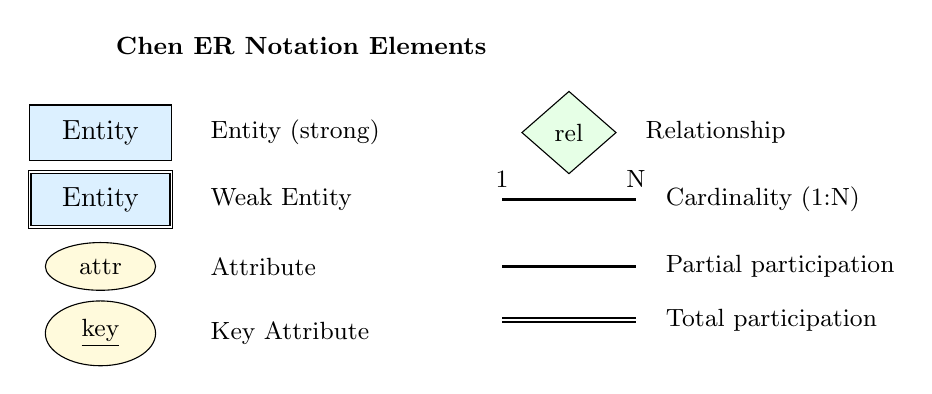
\begin{tikzpicture}[scale=0.85]
    % Legend
    \node[font=\small\bfseries] at (0, 4.5) {Chen ER Notation Elements};
    
    % Entity
    \node[draw, fill=entitycolor, minimum width=1.8cm, minimum height=0.7cm] at (-3, 3.2) {Entity};
    \node[right, font=\small] at (-1.5, 3.2) {Entity (strong)};
    
    % Weak Entity
    \node[draw, double, fill=entitycolor, minimum width=1.8cm, minimum height=0.7cm] at (-3, 2.2) {Entity};
    \node[right, font=\small] at (-1.5, 2.2) {Weak Entity};
    
    % Attribute
    \node[draw, ellipse, fill=attributecolor, minimum width=1.4cm, minimum height=0.6cm, font=\small] at (-3, 1.2) {attr};
    \node[right, font=\small] at (-1.5, 1.2) {Attribute};
    
    % Key Attribute
    \node[draw, ellipse, fill=attributecolor, minimum width=1.4cm, minimum height=0.6cm, font=\small] at (-3, 0.2) {\underline{key}};
    \node[right, font=\small] at (-1.5, 0.2) {Key Attribute};
    
    % Relationship
    \node[draw, diamond, fill=relationcolor, minimum width=1.2cm, minimum height=0.8cm, font=\small] at (4, 3.2) {rel};
    \node[right, font=\small] at (5, 3.2) {Relationship};
    
    % Cardinality
    \draw[thick] (3, 2.2) -- (5, 2.2);
    \node[font=\small] at (3, 2.5) {1};
    \node[font=\small] at (5, 2.5) {N};
    \node[right, font=\small] at (5.3, 2.2) {Cardinality (1:N)};
    
    % Participation
    \draw[thick] (3, 1.2) -- (5, 1.2);
    \node[right, font=\small] at (5.3, 1.2) {Partial participation};
    
    \draw[thick, double] (3, 0.4) -- (5, 0.4);
    \node[right, font=\small] at (5.3, 0.4) {Total participation};
\end{tikzpicture}
\caption{Chen ER Notation Legend}
\end{figure}

\subsubsection{Crow's Foot Notation}

\begin{figure}[H]
\centering
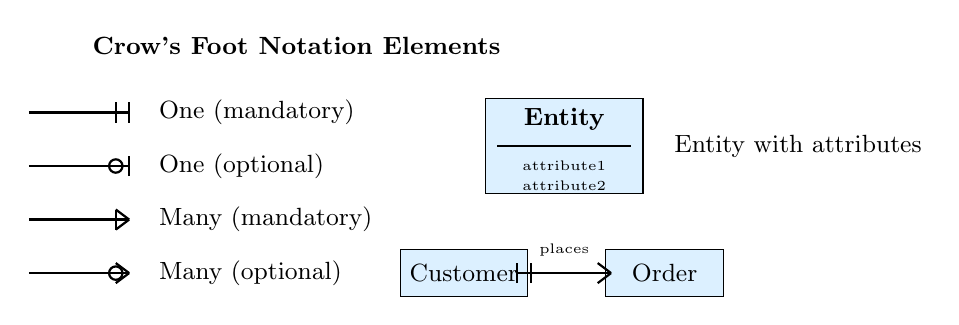
\begin{tikzpicture}[scale=0.85]
    % Legend
    \node[font=\small\bfseries] at (0, 4) {Crow's Foot Notation Elements};
    
    % One mandatory
    \draw[thick] (-4, 3) -- (-2.5, 3);
    \draw[thick] (-2.7, 2.85) -- (-2.7, 3.15);
    \draw[thick] (-2.5, 2.85) -- (-2.5, 3.15);
    \node[right, font=\small] at (-2.2, 3) {One (mandatory)};
    
    % One optional
    \draw[thick] (-4, 2.2) -- (-2.5, 2.2);
    \draw[thick] (-2.5, 2.05) -- (-2.5, 2.35);
    \draw[thick] (-2.7, 2.2) circle (0.1);
    \node[right, font=\small] at (-2.2, 2.2) {One (optional)};
    
    % Many mandatory
    \draw[thick] (-4, 1.4) -- (-2.5, 1.4);
    \draw[thick] (-2.7, 1.25) -- (-2.7, 1.55);
    \draw[thick] (-2.5, 1.4) -- (-2.7, 1.55);
    \draw[thick] (-2.5, 1.4) -- (-2.7, 1.25);
    \node[right, font=\small] at (-2.2, 1.4) {Many (mandatory)};
    
    % Many optional
    \draw[thick] (-4, 0.6) -- (-2.5, 0.6);
    \draw[thick] (-2.7, 0.6) circle (0.1);
    \draw[thick] (-2.5, 0.6) -- (-2.7, 0.75);
    \draw[thick] (-2.5, 0.6) -- (-2.7, 0.45);
    \node[right, font=\small] at (-2.2, 0.6) {Many (optional)};
    
    % Entity box
    \node[draw, fill=entitycolor, minimum width=2cm, minimum height=1.2cm] at (4, 2.5) {};
    \node[font=\small\bfseries] at (4, 2.9) {Entity};
    \draw[thick] (3, 2.5) -- (5, 2.5);
    \node[font=\tiny] at (4, 2.2) {attribute1};
    \node[font=\tiny] at (4, 1.9) {attribute2};
    \node[right, font=\small] at (5.5, 2.5) {Entity with attributes};
    
    % Example relationship
    \node[draw, fill=entitycolor, minimum width=1.5cm, minimum height=0.6cm, font=\small] at (2.5, 0.6) {Customer};
    \node[draw, fill=entitycolor, minimum width=1.5cm, minimum height=0.6cm, font=\small] at (5.5, 0.6) {Order};
    \draw[thick] (3.3, 0.6) -- (4.7, 0.6);
    \draw[thick] (3.5, 0.45) -- (3.5, 0.75);
    \draw[thick] (3.3, 0.45) -- (3.3, 0.75);
    \draw[thick] (4.7, 0.6) -- (4.5, 0.75);
    \draw[thick] (4.7, 0.6) -- (4.5, 0.45);
    \node[font=\tiny, above] at (4, 0.7) {places};
\end{tikzpicture}
\caption{Crow's Foot Notation Legend}
\end{figure}

\subsection{Data Flow Diagram Notation}

Data Flow Diagrams (DFDs) use standardized symbols to show data movement:

\begin{figure}[H]
\centering
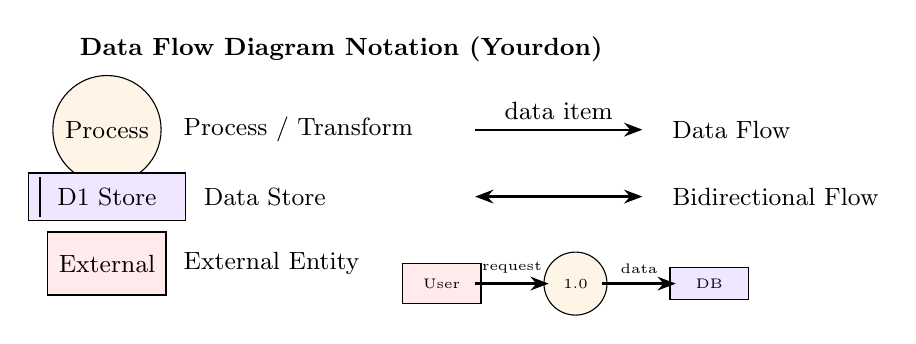
\begin{tikzpicture}[scale=0.85]
    % Legend
    \node[font=\small\bfseries] at (0, 4) {Data Flow Diagram Notation (Yourdon)};
    
    % Process
    \node[draw, circle, fill=processcolor, minimum size=1.2cm, font=\small] at (-3.5, 2.8) {Process};
    \node[right, font=\small] at (-2.5, 2.8) {Process / Transform};
    
    % Data Store
    \node[draw, fill=storecolor, minimum width=2cm, minimum height=0.6cm] at (-3.5, 1.8) {};
    \draw[thick] (-4.5, 1.5) -- (-4.5, 2.1);
    \node[font=\small] at (-3.5, 1.8) {D1 Store};
    \node[right, font=\small] at (-2.2, 1.8) {Data Store};
    
    % External Entity
    \node[draw, fill=flowcolor, minimum width=1.5cm, minimum height=0.8cm, font=\small] at (-3.5, 0.8) {External};
    \node[right, font=\small] at (-2.5, 0.8) {External Entity};
    
    % Data Flow
    \draw[-{Stealth}, thick] (2, 2.8) -- (4.5, 2.8);
    \node[above, font=\small] at (3.25, 2.8) {data item};
    \node[right, font=\small] at (4.8, 2.8) {Data Flow};
    
    % Bidirectional
    \draw[{Stealth}-{Stealth}, thick] (2, 1.8) -- (4.5, 1.8);
    \node[right, font=\small] at (4.8, 1.8) {Bidirectional Flow};
    
    % Example
    \node[draw, fill=flowcolor, minimum width=1cm, minimum height=0.5cm, font=\tiny] at (1.5, 0.5) {User};
    \node[draw, circle, fill=processcolor, minimum size=0.8cm, font=\tiny] at (3.5, 0.5) {1.0};
    \node[draw, fill=storecolor, minimum width=1cm, minimum height=0.4cm, font=\tiny] at (5.5, 0.5) {DB};
    \draw[-{Stealth}, thick] (2, 0.5) -- (3.1, 0.5) node[midway, above, font=\tiny] {request};
    \draw[-{Stealth}, thick] (3.9, 0.5) -- (5, 0.5) node[midway, above, font=\tiny] {data};
\end{tikzpicture}
\caption{Data Flow Diagram Notation Legend}
\end{figure}

\subsection{Data Definition Languages}

Physical data models are often expressed using database-specific DDL:

\begin{lstlisting}[caption={SQL DDL Example}, language=sql]
-- Customer entity
CREATE TABLE customer (
    customer_id     UUID PRIMARY KEY DEFAULT gen_random_uuid(),
    email           VARCHAR(255) NOT NULL UNIQUE,
    first_name      VARCHAR(100) NOT NULL,
    last_name       VARCHAR(100) NOT NULL,
    phone           VARCHAR(20),
    created_at      TIMESTAMP NOT NULL DEFAULT CURRENT_TIMESTAMP,
    updated_at      TIMESTAMP NOT NULL DEFAULT CURRENT_TIMESTAMP,
    status          VARCHAR(20) NOT NULL DEFAULT 'active'
        CHECK (status IN ('active', 'inactive', 'suspended')),
    
    -- Audit fields
    created_by      VARCHAR(100),
    updated_by      VARCHAR(100)
);

-- Order entity with foreign key
CREATE TABLE orders (
    order_id        UUID PRIMARY KEY DEFAULT gen_random_uuid(),
    customer_id     UUID NOT NULL REFERENCES customer(customer_id),
    order_date      TIMESTAMP NOT NULL DEFAULT CURRENT_TIMESTAMP,
    total_amount    DECIMAL(12,2) NOT NULL CHECK (total_amount >= 0),
    status          VARCHAR(20) NOT NULL DEFAULT 'pending'
        CHECK (status IN ('pending', 'confirmed', 'shipped', 'delivered', 'cancelled')),
    
    -- Indexing for common queries
    INDEX idx_customer_orders (customer_id),
    INDEX idx_order_date (order_date)
);
\end{lstlisting}

\subsection{Data Catalog Specifications}

Data catalogs document metadata about data assets:

\begin{table}[H]
\centering
\caption{Example Data Catalog Entry Format}
\small
\begin{tabular}{@{}L{3cm}L{10.5cm}@{}}
\toprule
\textbf{Attribute} & \textbf{Value} \\
\midrule
\textbf{Asset Name} & customer \\
\textbf{Type} & Table \\
\textbf{Database} & commerce\_db \\
\textbf{Schema} & public \\
\textbf{Owner} & Customer Domain Team \\
\textbf{Steward} & Jane Smith \\
\textbf{Classification} & Confidential - PII \\
\textbf{Description} & Master customer records containing profile and contact information \\
\textbf{Retention} & 7 years after last activity \\
\textbf{Update Frequency} & Real-time \\
\textbf{Row Count} & ~2.5M \\
\textbf{Quality Score} & 94\% \\
\textbf{Tags} & customer, profile, PII, master-data \\
\bottomrule
\end{tabular}
\end{table}

\subsection{Tabular Specifications}

\subsubsection{Entity Attribute Table}

\begin{table}[H]
\centering
\caption{Example Entity Attribute Specification}
\small
\begin{tabular}{@{}L{2.2cm}L{2cm}L{1.5cm}L{1.3cm}L{2cm}L{3.5cm}@{}}
\toprule
\textbf{Attribute} & \textbf{Data Type} & \textbf{Nullable} & \textbf{Key} & \textbf{Default} & \textbf{Description} \\
\midrule
customer\_id & UUID & No & PK & auto-gen & Unique identifier \\
email & VARCHAR(255) & No & UK & -- & Email address \\
first\_name & VARCHAR(100) & No & -- & -- & First name \\
last\_name & VARCHAR(100) & No & -- & -- & Last name \\
phone & VARCHAR(20) & Yes & -- & NULL & Phone number \\
status & VARCHAR(20) & No & -- & 'active' & Account status \\
created\_at & TIMESTAMP & No & -- & NOW() & Creation time \\
\bottomrule
\end{tabular}
\end{table}

\subsubsection{Data Quality Rules Table}

\begin{table}[H]
\centering
\caption{Example Data Quality Rules Specification}
\small
\begin{tabular}{@{}L{1.5cm}L{2cm}L{2cm}L{4cm}L{2cm}L{1.5cm}@{}}
\toprule
\textbf{Rule ID} & \textbf{Entity} & \textbf{Attribute} & \textbf{Rule} & \textbf{Severity} & \textbf{Action} \\
\midrule
DQ-001 & Customer & email & Valid email format & Critical & Reject \\
DQ-002 & Customer & phone & Valid phone format & Warning & Flag \\
DQ-003 & Order & total & Must be >= 0 & Critical & Reject \\
DQ-004 & Order & customer\_id & Must exist in Customer & Critical & Reject \\
DQ-005 & Product & price & Within expected range & Warning & Review \\
\bottomrule
\end{tabular}
\end{table}

% =============================================================================
% SECTION: VIEWPOINT METAMODELS
% =============================================================================
\section{Viewpoint Metamodels}

This section defines the conceptual metamodel underlying the Information Viewpoint, establishing the vocabulary of element types, their properties, and valid relationships.

\subsection{Core Metamodel}

\begin{figure}[H]
\centering
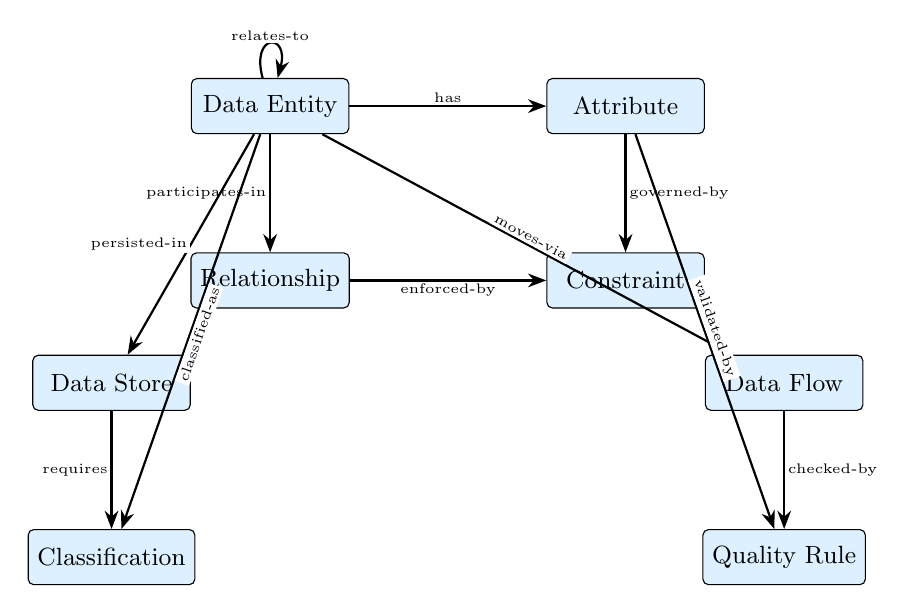
\begin{tikzpicture}[
    node distance=1.3cm and 2cm,
    entity/.style={draw, fill=entitycolor, rounded corners=2pt, minimum width=2cm, minimum height=0.7cm, font=\small},
    arrow/.style={-{Stealth}, thick},
    label/.style={font=\tiny, fill=white, inner sep=1pt}
]
    % Main entities
    \node[entity] (dataentity) {Data Entity};
    \node[entity, right=2.5cm of dataentity] (attribute) {Attribute};
    \node[entity, below=1.5cm of dataentity] (relationship) {Relationship};
    \node[entity, below=1.5cm of attribute] (constraint) {Constraint};
    \node[entity, below left=2.8cm and 0cm of dataentity] (datastore) {Data Store};
    \node[entity, below right=2.8cm and 0cm of attribute] (dataflow) {Data Flow};
    \node[entity, below=1.5cm of datastore] (classification) {Classification};
    \node[entity, below=1.5cm of dataflow] (qualityrule) {Quality Rule};
    
    % Relationships
    \draw[arrow] (dataentity) -- (attribute) node[label, midway, above] {has};
    \draw[arrow] (dataentity) -- (relationship) node[label, midway, left] {participates-in};
    \draw[arrow] (attribute) -- (constraint) node[label, midway, right] {governed-by};
    \draw[arrow] (dataentity) -- (datastore) node[label, midway, left] {persisted-in};
    \draw[arrow] (dataentity) -- (dataflow) node[label, midway, above, sloped] {moves-via};
    \draw[arrow] (dataentity) -- (classification) node[label, midway, below, sloped] {classified-as};
    \draw[arrow] (attribute) -- (qualityrule) node[label, midway, above, sloped] {validated-by};
    \draw[arrow] (relationship) -- (constraint) node[label, midway, below] {enforced-by};
    \draw[arrow] (datastore) -- (classification) node[label, midway, left] {requires};
    \draw[arrow] (dataflow) -- (qualityrule) node[label, midway, right] {checked-by};
    
    % Self-reference
    \draw[arrow] (dataentity) to[loop above] node[label, above] {relates-to} (dataentity);
\end{tikzpicture}
\caption{Information Viewpoint Core Metamodel}
\end{figure}

\subsection{Entity Definitions}

\begin{definitionbox}[Entity: Data Entity]
\textbf{Definition:} A distinguishable object or concept about which data is captured and stored. Represents a business object, event, or concept of interest.

\textbf{Attributes:}
\begin{itemize}[nosep]
    \item \texttt{entityId}: Unique identifier for the entity
    \item \texttt{name}: Business name for the entity
    \item \texttt{description}: Detailed business description
    \item \texttt{type}: Entity type (master, transactional, reference, derived)
    \item \texttt{domain}: Business domain ownership
    \item \texttt{version}: Schema version
    \item \texttt{status}: Lifecycle status (draft, active, deprecated)
    \item \texttt{aliases}: Alternative names or synonyms
    \item \texttt{businessRules}: Associated business rules
\end{itemize}

\textbf{Constraints:}
\begin{itemize}[nosep]
    \item Each entity must have a unique identifier attribute
    \item Entity names must be unique within a domain
    \item Entities must be assigned to exactly one owning domain
    \item Master entities must have defined golden record rules
\end{itemize}
\end{definitionbox}

\begin{definitionbox}[Entity: Attribute]
\textbf{Definition:} A property or characteristic of a data entity that captures a specific piece of information.

\textbf{Attributes:}
\begin{itemize}[nosep]
    \item \texttt{attributeId}: Unique identifier
    \item \texttt{name}: Attribute name (following naming standards)
    \item \texttt{description}: Business meaning
    \item \texttt{dataType}: Logical data type
    \item \texttt{length}: Maximum length (if applicable)
    \item \texttt{precision}: Numeric precision (if applicable)
    \item \texttt{nullable}: Whether null values are allowed
    \item \texttt{defaultValue}: Default value if not provided
    \item \texttt{keyType}: Key classification (PK, FK, AK, none)
    \item \texttt{sensitivity}: Data sensitivity classification
    \item \texttt{piiFlag}: Whether attribute contains PII
\end{itemize}

\textbf{Constraints:}
\begin{itemize}[nosep]
    \item Attribute names must be unique within an entity
    \item Data types must be from approved type list
    \item PII attributes must have appropriate classification
    \item Key attributes cannot be nullable
\end{itemize}
\end{definitionbox}

\begin{definitionbox}[Entity: Relationship]
\textbf{Definition:} An association between two or more data entities that captures a business rule or structural connection.

\textbf{Attributes:}
\begin{itemize}[nosep]
    \item \texttt{relationshipId}: Unique identifier
    \item \texttt{name}: Relationship name (verb phrase)
    \item \texttt{description}: Business meaning of relationship
    \item \texttt{sourceEntity}: Origin entity
    \item \texttt{targetEntity}: Destination entity
    \item \texttt{sourceCardinality}: Cardinality at source (1, 0..1, *, 1..*)
    \item \texttt{targetCardinality}: Cardinality at target
    \item \texttt{type}: Relationship type (association, aggregation, composition, generalization)
    \item \texttt{mandatory}: Whether relationship is required
    \item \texttt{bidirectional}: Whether navigable both directions
\end{itemize}

\textbf{Constraints:}
\begin{itemize}[nosep]
    \item Many-to-many relationships require junction entities
    \item Composition relationships imply cascade delete
    \item Circular relationships must be explicitly justified
\end{itemize}
\end{definitionbox}

\begin{definitionbox}[Entity: Data Store]
\textbf{Definition:} A persistent storage mechanism that holds data entities, such as a database, file system, or data lake.

\textbf{Attributes:}
\begin{itemize}[nosep]
    \item \texttt{storeId}: Unique identifier
    \item \texttt{name}: Store name
    \item \texttt{type}: Storage technology (RDBMS, NoSQL, Object, File)
    \item \texttt{technology}: Specific product (PostgreSQL, MongoDB, S3)
    \item \texttt{environment}: Deployment environment
    \item \texttt{connectionInfo}: Connection parameters
    \item \texttt{capacity}: Storage capacity
    \item \texttt{retentionPolicy}: Data retention configuration
    \item \texttt{backupPolicy}: Backup configuration
    \item \texttt{encryptionConfig}: Encryption settings
\end{itemize}

\textbf{Constraints:}
\begin{itemize}[nosep]
    \item Production stores must have backup policies
    \item Stores with PII must have encryption enabled
    \item Connection credentials must be stored securely
\end{itemize}
\end{definitionbox}

\begin{definitionbox}[Entity: Data Flow]
\textbf{Definition:} A movement of data between system components, processes, or data stores, including any transformations applied.

\textbf{Attributes:}
\begin{itemize}[nosep]
    \item \texttt{flowId}: Unique identifier
    \item \texttt{name}: Flow name
    \item \texttt{description}: Purpose of the data flow
    \item \texttt{source}: Origin component or store
    \item \texttt{target}: Destination component or store
    \item \texttt{dataElements}: Data items in the flow
    \item \texttt{frequency}: Flow frequency (real-time, batch, on-demand)
    \item \texttt{volume}: Expected data volume
    \item \texttt{transformations}: Transformations applied
    \item \texttt{protocol}: Transport protocol
    \item \texttt{errorHandling}: Error handling strategy
\end{itemize}

\textbf{Constraints:}
\begin{itemize}[nosep]
    \item Flows must specify error handling behavior
    \item Cross-boundary flows must be encrypted
    \item High-volume flows must have capacity planning
\end{itemize}
\end{definitionbox}

\begin{definitionbox}[Entity: Classification]
\textbf{Definition:} A categorization of data based on sensitivity, regulatory requirements, or business importance.

\textbf{Attributes:}
\begin{itemize}[nosep]
    \item \texttt{classificationId}: Unique identifier
    \item \texttt{level}: Classification level (Public, Internal, Confidential, Restricted)
    \item \texttt{category}: Data category (PII, PHI, PCI, Financial, IP)
    \item \texttt{handlingRequirements}: Required handling procedures
    \item \texttt{encryptionRequired}: Whether encryption is mandated
    \item \texttt{accessRestrictions}: Access control requirements
    \item \texttt{retentionRequirements}: Retention period requirements
    \item \texttt{regulatoryBasis}: Applicable regulations
\end{itemize}

\textbf{Constraints:}
\begin{itemize}[nosep]
    \item Higher classifications inherit lower classification requirements
    \item PII classification requires GDPR/CCPA compliance measures
    \item Restricted data requires audit logging
\end{itemize}
\end{definitionbox}

\begin{definitionbox}[Entity: Quality Rule]
\textbf{Definition:} A specification of a data quality requirement that data must satisfy, including validation logic and remediation actions.

\textbf{Attributes:}
\begin{itemize}[nosep]
    \item \texttt{ruleId}: Unique identifier
    \item \texttt{name}: Rule name
    \item \texttt{description}: Business rationale
    \item \texttt{dimension}: Quality dimension (accuracy, completeness, consistency, timeliness, validity, uniqueness)
    \item \texttt{expression}: Rule logic/expression
    \item \texttt{severity}: Violation severity (critical, major, minor, warning)
    \item \texttt{threshold}: Acceptable threshold
    \item \texttt{action}: Action on violation (reject, flag, correct, notify)
    \item \texttt{owner}: Rule owner
\end{itemize}

\textbf{Constraints:}
\begin{itemize}[nosep]
    \item Critical rules must have defined remediation procedures
    \item Rules must be testable and measurable
    \item Rule ownership must be assigned
\end{itemize}
\end{definitionbox}

\begin{definitionbox}[Entity: Constraint]
\textbf{Definition:} A rule or restriction that governs the values, relationships, or behavior of data elements.

\textbf{Attributes:}
\begin{itemize}[nosep]
    \item \texttt{constraintId}: Unique identifier
    \item \texttt{name}: Constraint name
    \item \texttt{type}: Constraint type (primary key, foreign key, unique, check, not null, default)
    \item \texttt{expression}: Constraint definition
    \item \texttt{scope}: Affected elements
    \item \texttt{enforcement}: Enforcement timing (immediate, deferred)
    \item \texttt{violationAction}: Action on violation
\end{itemize}

\textbf{Constraints:}
\begin{itemize}[nosep]
    \item Primary key constraints must be non-null and unique
    \item Foreign key constraints must reference existing keys
    \item Check constraints must be deterministic
\end{itemize}
\end{definitionbox}

\subsection{Relationship Definitions}

\begin{table}[H]
\centering
\caption{Metamodel Relationship Definitions}
\small
\begin{tabular}{@{}L{2.3cm}L{1.8cm}L{1.8cm}L{7.5cm}@{}}
\toprule
\textbf{Relationship} & \textbf{Source} & \textbf{Target} & \textbf{Description} \\
\midrule
has & Data Entity & Attribute & Entity contains this attribute \\
\addlinespace
participates-in & Data Entity & Relationship & Entity is involved in this relationship \\
\addlinespace
governed-by & Attribute & Constraint & Attribute is restricted by constraint \\
\addlinespace
persisted-in & Data Entity & Data Store & Entity data is stored here \\
\addlinespace
moves-via & Data Entity & Data Flow & Entity data transfers through this flow \\
\addlinespace
classified-as & Data Entity & Classification & Entity has this sensitivity level \\
\addlinespace
validated-by & Attribute & Quality Rule & Attribute is checked by this rule \\
\addlinespace
derives-from & Data Entity & Data Entity & Entity is computed from source entity \\
\addlinespace
masters & Data Entity & Data Entity & Entity is authoritative source \\
\addlinespace
transforms & Data Flow & Data Entity & Flow modifies entity data \\
\bottomrule
\end{tabular}
\end{table}

% =============================================================================
% SECTION: CONFORMING NOTATIONS
% =============================================================================
\section{Conforming Notations}

Several existing notations and modeling languages conform to the Information Viewpoint metamodel.

\subsection{Entity-Relationship Diagrams}

ER diagrams in various notations (Chen, Crow's Foot, IDEF1X, Barker) are the primary notation for data modeling.

\textbf{Conformance Level:} Full conformance for structural data modeling.

\textbf{Tool Support:} ERwin, PowerDesigner, Lucidchart, draw.io, MySQL Workbench, pgModeler.

\subsection{UML Class Diagrams}

UML class diagrams can represent data models, particularly when modeling object-relational mappings.

\textbf{Conformance Level:} Partial conformance; better for object models than relational.

\textbf{Tool Support:} Enterprise Architect, Visual Paradigm, StarUML, PlantUML.

\subsection{Data Flow Diagrams}

DFDs (Yourdon/DeMarco, Gane-Sarson) show data movement through systems.

\textbf{Conformance Level:} Full conformance for flow modeling.

\textbf{Tool Support:} Lucidchart, draw.io, Visio, SmartDraw.

\subsection{BPMN Data Objects}

BPMN includes data object notation that can document data in process context.

\textbf{Conformance Level:} Partial conformance; process-centric focus.

\textbf{Tool Support:} Camunda, Bizagi, Signavio, ARIS.

\subsection{Data Catalog Tools}

Modern data catalog platforms provide comprehensive data documentation:

\begin{table}[H]
\centering
\caption{Data Catalog and Governance Tools}
\small
\begin{tabular}{@{}L{3cm}L{3.5cm}L{7cm}@{}}
\toprule
\textbf{Tool} & \textbf{Type} & \textbf{Key Capabilities} \\
\midrule
Collibra & Data Governance & Catalog, lineage, quality, stewardship \\
Alation & Data Catalog & Discovery, collaboration, governance \\
Apache Atlas & Open Source & Metadata, lineage, classification (Hadoop) \\
AWS Glue Catalog & Cloud Native & Schema discovery, ETL integration \\
Azure Purview & Cloud Native & Unified governance across Azure \\
dbt & Transform Tool & Documentation, lineage, testing \\
Great Expectations & Quality & Data validation, documentation \\
DataHub & Open Source & Metadata search, lineage, discovery \\
\bottomrule
\end{tabular}
\end{table}

\begin{table}[H]
\centering
\caption{Notation Comparison Matrix}
\footnotesize
\begin{tabular}{@{}L{2.5cm}C{1cm}C{1cm}C{1cm}C{1cm}C{1cm}C{1cm}C{1cm}@{}}
\toprule
\textbf{Feature} & \rotatebox{60}{\textbf{Chen ER}} & \rotatebox{60}{\textbf{Crow's Foot}} & \rotatebox{60}{\textbf{UML}} & \rotatebox{60}{\textbf{DFD}} & \rotatebox{60}{\textbf{BPMN}} & \rotatebox{60}{\textbf{Catalog}} & \rotatebox{60}{\textbf{Custom}} \\
\midrule
Entities & $\bullet$ & $\bullet$ & $\bullet$ & $\circ$ & $\circ$ & $\bullet$ & $\bullet$ \\
Attributes & $\bullet$ & $\bullet$ & $\bullet$ & -- & -- & $\bullet$ & $\bullet$ \\
Relationships & $\bullet$ & $\bullet$ & $\bullet$ & -- & $\circ$ & $\bullet$ & $\bullet$ \\
Cardinality & $\bullet$ & $\bullet$ & $\bullet$ & -- & -- & $\circ$ & $\bullet$ \\
Data Flow & -- & -- & $\circ$ & $\bullet$ & $\bullet$ & $\circ$ & $\bullet$ \\
Classification & -- & -- & $\circ$ & -- & -- & $\bullet$ & $\bullet$ \\
Lineage & -- & -- & -- & $\circ$ & $\circ$ & $\bullet$ & $\bullet$ \\
Quality Rules & -- & -- & $\circ$ & -- & -- & $\bullet$ & $\bullet$ \\
Standardized & $\bullet$ & $\bullet$ & $\bullet$ & $\bullet$ & $\bullet$ & -- & -- \\
\bottomrule
\multicolumn{8}{l}{\footnotesize $\bullet$ = Strong support, $\circ$ = Limited support, -- = Not applicable}
\end{tabular}
\end{table}

% =============================================================================
% SECTION: MODEL CORRESPONDENCE RULES
% =============================================================================
\section{Model Correspondence Rules}

Model correspondence rules define how elements in information models relate to elements in other architectural views.

\subsection{Development View Correspondence}

\begin{definitionbox}[Correspondence Rule CR-01: Entity to Class Mapping]
\textbf{Rule:} Each data entity in the logical model should correspond to one or more domain classes in the development view.

\textbf{Formal Expression:}
\begin{center}
$\forall e \in DataEntities : \exists C \subseteq Classes : implements(C, e)$
\end{center}

\textbf{Rationale:} Ensures data structures are properly implemented in code.

\textbf{Verification:} ORM mapping review, code inspection.
\end{definitionbox}

\begin{definitionbox}[Correspondence Rule CR-02: Attribute to Property Mapping]
\textbf{Rule:} Each attribute in a data entity must map to a property in the corresponding domain class with compatible type.

\textbf{Formal Expression:}
\begin{center}
$\forall a \in entity.attributes : \exists p \in class.properties : maps(a, p) \land compatible(a.type, p.type)$
\end{center}

\textbf{Rationale:} Ensures complete and type-safe data mapping.

\textbf{Verification:} ORM configuration audit.
\end{definitionbox}

\subsection{Component-and-Connector View Correspondence}

\begin{definitionbox}[Correspondence Rule CR-03: Data Store to Component Mapping]
\textbf{Rule:} Each data store in the information model must correspond to a component in the C\&C view.

\textbf{Formal Expression:}
\begin{center}
$\forall ds \in DataStores : \exists c \in Components : realizes(c, ds)$
\end{center}

\textbf{Rationale:} Ensures all storage is architecturally represented.

\textbf{Verification:} C\&C diagram review.
\end{definitionbox}

\begin{definitionbox}[Correspondence Rule CR-04: Data Flow to Connector Mapping]
\textbf{Rule:} Data flows crossing component boundaries must have corresponding connectors in the C\&C view.

\textbf{Formal Expression:}
\begin{center}
$\forall df \in DataFlows : crossesBoundary(df) \Rightarrow \exists conn \in Connectors : carries(conn, df)$
\end{center}

\textbf{Rationale:} Ensures data movement is architecturally visible.

\textbf{Verification:} Flow-connector mapping matrix.
\end{definitionbox}

\subsection{Deployment View Correspondence}

\begin{definitionbox}[Correspondence Rule CR-05: Data Store to Infrastructure Mapping]
\textbf{Rule:} Each data store must be allocated to deployment infrastructure in the deployment view.

\textbf{Formal Expression:}
\begin{center}
$\forall ds \in DataStores : \exists n \in Nodes : hosts(n, ds)$
\end{center}

\textbf{Rationale:} Ensures all data has defined physical location.

\textbf{Verification:} Deployment diagram audit.
\end{definitionbox}

\subsection{Security View Correspondence}

\begin{definitionbox}[Correspondence Rule CR-06: Classification to Security Control Mapping]
\textbf{Rule:} Each data classification level must have corresponding security controls implemented.

\textbf{Formal Expression:}
\begin{center}
$\forall c \in Classifications : \exists S \subseteq SecurityControls : protects(S, c)$
\end{center}

\textbf{Rationale:} Ensures security requirements are implemented.

\textbf{Verification:} Security control assessment.
\end{definitionbox}

\subsection{Correspondence Verification Matrix}

\begin{table}[H]
\centering
\caption{Cross-View Correspondence Verification}
\small
\begin{tabular}{@{}L{2.3cm}L{3.2cm}L{3.2cm}L{4cm}@{}}
\toprule
\textbf{Rule ID} & \textbf{Source View} & \textbf{Target Elements} & \textbf{Verification Method} \\
\midrule
CR-01 & Data Entities & Domain Classes & ORM mapping review \\
CR-02 & Attributes & Class Properties & Type compatibility check \\
CR-03 & Data Stores & C\&C Components & Diagram alignment \\
CR-04 & Data Flows & Connectors & Flow-connector mapping \\
CR-05 & Data Stores & Infrastructure Nodes & Deployment audit \\
CR-06 & Classifications & Security Controls & Control assessment \\
\bottomrule
\end{tabular}
\end{table}

% =============================================================================
% SECTION: OPERATIONS ON VIEWS
% =============================================================================
\section{Operations on Views}

This section defines the methods and procedures for creating, interpreting, analyzing, and implementing information views.

\subsection{Creation Methods}

\subsubsection{View Development Process}

\begin{guidancebox}[Step 1: Establish Context and Scope]
\begin{enumerate}[nosep]
    \item Identify business domains and subject areas
    \item Gather business requirements and use cases
    \item Review existing data assets and systems
    \item Identify key stakeholders and data owners
    \item Define scope boundaries for the data model
\end{enumerate}
\end{guidancebox}

\begin{guidancebox}[Step 2: Develop Conceptual Data Model]
\begin{enumerate}[nosep]
    \item Identify business entities from requirements
    \item Define entity relationships using business terms
    \item Validate with business stakeholders
    \item Document business rules affecting data
    \item Establish entity ownership by domain
\end{enumerate}
\end{guidancebox}

\begin{guidancebox}[Step 3: Develop Logical Data Model]
\begin{enumerate}[nosep]
    \item Refine entities with full attribute definitions
    \item Normalize to appropriate normal form (typically 3NF)
    \item Define primary and foreign keys
    \item Specify data types and constraints
    \item Document cardinality and optionality
    \item Resolve many-to-many relationships
\end{enumerate}
\end{guidancebox}

\begin{guidancebox}[Step 4: Define Data Flows]
\begin{enumerate}[nosep]
    \item Identify data sources (internal and external)
    \item Map data movement between systems
    \item Document transformations applied
    \item Specify integration patterns (ETL, API, CDC)
    \item Define error handling and recovery
\end{enumerate}
\end{guidancebox}

\begin{guidancebox}[Step 5: Establish Data Governance]
\begin{enumerate}[nosep]
    \item Classify data by sensitivity
    \item Define data quality rules
    \item Establish retention policies
    \item Document compliance requirements
    \item Assign data stewardship responsibilities
\end{enumerate}
\end{guidancebox}

\begin{guidancebox}[Step 6: Develop Physical Data Model]
\begin{enumerate}[nosep]
    \item Select storage technologies
    \item Denormalize for performance where justified
    \item Define indexes and partitioning strategies
    \item Specify physical constraints
    \item Plan storage capacity
    \item Generate DDL scripts
\end{enumerate}
\end{guidancebox}

\begin{guidancebox}[Step 7: Validate and Review]
\begin{enumerate}[nosep]
    \item Verify alignment with requirements
    \item Check correspondence with other views
    \item Review with data architects and DBAs
    \item Validate security and compliance
    \item Document rationale for key decisions
\end{enumerate}
\end{guidancebox}

\subsubsection{Documentation Templates}

\textbf{Entity Specification Template:}

\begin{lstlisting}[caption={Entity Specification Template}, language={}]
Entity Specification
====================
Entity ID:       [ENT-XXX]
Name:            [Entity Name]
Domain:          [Business Domain]
Type:            [Master | Transactional | Reference | Derived]
Status:          [Draft | Active | Deprecated]

Business Description:
  [Detailed business meaning and purpose]

Attributes:
  +---------------+----------+------+-----+---------+-------------------+
  | Name          | Type     | Null | Key | Default | Description       |
  +---------------+----------+------+-----+---------+-------------------+
  | [attr_name]   | [type]   | Y/N  | PK  | [value] | [description]     |
  +---------------+----------+------+-----+---------+-------------------+

Relationships:
  - [Relationship Name]: [Target Entity] ([Cardinality])
  - ...

Constraints:
  - [Constraint Name]: [Definition]
  - ...

Data Classification:
  - Sensitivity:     [Public | Internal | Confidential | Restricted]
  - Contains PII:    [Yes/No]
  - Regulations:     [GDPR, CCPA, HIPAA, PCI-DSS, etc.]

Quality Rules:
  - [Rule ID]: [Rule Description]
  - ...

Lifecycle:
  - Creation:        [How data is created]
  - Retention:       [Retention period]
  - Archival:        [Archival policy]
  - Deletion:        [Deletion policy]

Owner:              [Data Owner]
Steward:            [Data Steward]
Last Updated:       [Date]
\end{lstlisting}

\subsubsection{Common Patterns and Idioms}

\begin{patternbox}[Pattern: Slowly Changing Dimension (SCD)]
\textbf{Context:} Need to track historical changes to reference data over time.

\textbf{Solution:} Implement versioning strategy for dimensional data.

\textbf{Types:}
\begin{itemize}[nosep]
    \item \textbf{Type 1:} Overwrite old value (no history)
    \item \textbf{Type 2:} Add new row with version/date range (full history)
    \item \textbf{Type 3:} Add new column for previous value (limited history)
    \item \textbf{Type 4:} Separate history table (full history, separate)
    \item \textbf{Type 6:} Hybrid combining Types 1, 2, and 3
\end{itemize}

\textbf{Use When:} Audit requirements, historical reporting, trend analysis.
\end{patternbox}

\begin{patternbox}[Pattern: Event Sourcing]
\textbf{Context:} Need complete audit trail and ability to reconstruct state.

\textbf{Solution:} Store all state changes as a sequence of events rather than current state only.

\textbf{Characteristics:}
\begin{itemize}[nosep]
    \item Events are immutable and append-only
    \item Current state derived by replaying events
    \item Complete audit history preserved
    \item Enables temporal queries and debugging
\end{itemize}

\textbf{Use When:} Financial systems, compliance requirements, complex business logic.
\end{patternbox}

\begin{patternbox}[Pattern: Data Vault]
\textbf{Context:} Enterprise data warehouse requiring flexibility and audit capability.

\textbf{Solution:} Model data using Hubs (business keys), Links (relationships), and Satellites (descriptive attributes).

\textbf{Components:}
\begin{itemize}[nosep]
    \item \textbf{Hub:} Unique business keys with load metadata
    \item \textbf{Link:} Relationships between hubs
    \item \textbf{Satellite:} Descriptive attributes with temporal tracking
\end{itemize}

\textbf{Use When:} Data warehouse, multiple source integration, changing requirements.
\end{patternbox}

\begin{patternbox}[Pattern: Polyglot Persistence]
\textbf{Context:} Different data types have different storage requirements.

\textbf{Solution:} Use different database technologies for different data needs.

\textbf{Typical Combinations:}
\begin{itemize}[nosep]
    \item RDBMS for transactional data with ACID requirements
    \item Document store for flexible schemas and nested data
    \item Graph database for highly connected data
    \item Time-series database for metrics and events
    \item Search engine for full-text search
    \item Cache for hot data and session state
\end{itemize}

\textbf{Use When:} Diverse data requirements, performance optimization needs.
\end{patternbox}

\begin{table}[H]
\centering
\caption{Data Modeling Patterns Summary}
\small
\begin{tabular}{@{}L{3cm}L{4.5cm}L{5.5cm}@{}}
\toprule
\textbf{Pattern} & \textbf{Description} & \textbf{Use When} \\
\midrule
Surrogate Key & System-generated ID separate from business key & Integration, performance, privacy \\
\addlinespace
Audit Columns & Standard columns for tracking changes & Compliance, debugging \\
\addlinespace
Soft Delete & Flag records as deleted rather than removing & Recovery, audit requirements \\
\addlinespace
Temporal Tables & Built-in versioning with valid time & Historical queries, audit \\
\addlinespace
Sharding & Horizontal partitioning across servers & High volume, scalability \\
\addlinespace
CQRS & Separate read and write models & Complex domains, scalability \\
\addlinespace
Materialized Views & Pre-computed query results & Performance, complex aggregations \\
\bottomrule
\end{tabular}
\end{table}

\subsection{Interpretive Methods}

\subsubsection{Reading Data Models}

When interpreting an information view, stakeholders should follow this systematic approach:

\begin{enumerate}
    \item \textbf{Understand the Scope:} Identify what subject area or domain is modeled and at what level of abstraction (conceptual, logical, physical).
    
    \item \textbf{Identify Key Entities:} Locate the central business entities and understand their purpose and ownership.
    
    \item \textbf{Trace Relationships:} Follow relationships between entities, noting cardinality and optionality to understand business rules.
    
    \item \textbf{Examine Attributes:} Review attribute definitions, data types, and constraints to understand what data is captured.
    
    \item \textbf{Check Classifications:} Identify sensitive data and understand applicable security and compliance requirements.
    
    \item \textbf{Follow Data Flows:} If flow diagrams are present, trace data movement to understand integration and transformation.
    
    \item \textbf{Review Quality Rules:} Understand what validation and quality constraints apply to the data.
\end{enumerate}

\subsubsection{Stakeholder-Specific Interpretation Guides}

\textbf{For Business Analysts:}
Focus on the conceptual model and business entity definitions. Verify that business concepts are correctly represented and relationships reflect actual business rules.

\textbf{For Developers:}
Examine the logical model for domain class design. Understand attribute types for ORM mapping. Note constraints that must be enforced in code.

\textbf{For DBAs:}
Review the physical model for implementation details. Assess indexing strategies, partitioning schemes, and storage requirements.

\textbf{For Data Scientists:}
Identify available data elements and their meaning. Understand data quality characteristics and any transformations applied.

\subsection{Analysis Methods}

\subsubsection{Data Model Quality Analysis}

\begin{definitionbox}[Normalization Analysis]
\textbf{Purpose:} Assess data model adherence to normal forms.

\textbf{Process:}
\begin{enumerate}[nosep]
    \item Check 1NF: Atomic values, no repeating groups
    \item Check 2NF: No partial dependencies on composite keys
    \item Check 3NF: No transitive dependencies
    \item Check BCNF: Every determinant is a candidate key
    \item Document justified denormalizations
\end{enumerate}

\textbf{Outputs:}
\begin{itemize}[nosep]
    \item Normal form assessment per entity
    \item Identified anomalies and redundancies
    \item Denormalization justifications
\end{itemize}
\end{definitionbox}

\subsubsection{Data Quality Assessment}

\begin{definitionbox}[Data Quality Dimension Analysis]
\textbf{Purpose:} Measure data quality across standard dimensions.

\textbf{Dimensions:}
\begin{itemize}[nosep]
    \item \textbf{Accuracy:} Data correctly represents real-world values
    \item \textbf{Completeness:} Required data is present
    \item \textbf{Consistency:} Data agrees across systems/time
    \item \textbf{Timeliness:} Data is current and available when needed
    \item \textbf{Validity:} Data conforms to defined formats/rules
    \item \textbf{Uniqueness:} No unintended duplicate records
\end{itemize}

\textbf{Outputs:}
\begin{itemize}[nosep]
    \item Quality scores by dimension and entity
    \item Identified quality issues
    \item Remediation recommendations
\end{itemize}
\end{definitionbox}

\subsubsection{Data Lineage Analysis}

\begin{definitionbox}[Lineage Impact Analysis]
\textbf{Purpose:} Understand data dependencies and change impact.

\textbf{Inputs:}
\begin{itemize}[nosep]
    \item Data lineage graph
    \item Element to be changed
    \item Type of change
\end{itemize}

\textbf{Process:}
\begin{enumerate}[nosep]
    \item Identify source element in lineage
    \item Trace all downstream dependencies
    \item Classify impact (schema, logic, reports)
    \item Identify affected systems and teams
    \item Estimate remediation scope
\end{enumerate}

\textbf{Outputs:}
\begin{itemize}[nosep]
    \item Downstream impact list
    \item Affected systems and processes
    \item Change coordination requirements
\end{itemize}
\end{definitionbox}

\subsection{Implementation Methods}

\subsubsection{Physical Implementation}

Translating data models to physical implementations follows established practices:

\begin{table}[H]
\centering
\caption{Implementation Mapping by Technology}
\small
\begin{tabular}{@{}L{2.5cm}L{2.5cm}L{4cm}L{4cm}@{}}
\toprule
\textbf{Technology} & \textbf{Entity Maps To} & \textbf{Relationship Maps To} & \textbf{Constraint Maps To} \\
\midrule
RDBMS & Table & Foreign Key & CHECK, UNIQUE, NOT NULL \\
Document DB & Collection & Embedded/Reference & Validation Schema \\
Graph DB & Node & Edge & Property Constraints \\
Key-Value & Key Prefix & Key Structure & Application Logic \\
Time-Series & Measurement & Tags/Fields & Retention Policies \\
\bottomrule
\end{tabular}
\end{table}

\subsubsection{Data Governance Implementation}

\begin{table}[H]
\centering
\caption{Governance Control Implementation}
\small
\begin{tabular}{@{}L{3cm}L{4cm}L{6cm}@{}}
\toprule
\textbf{Control Area} & \textbf{Mechanisms} & \textbf{Tools} \\
\midrule
Access Control & RBAC, ABAC, Row-level security & Database permissions, IAM policies \\
Encryption & TDE, Column-level, TLS & Database encryption, KMS \\
Masking & Dynamic, Static & Data masking tools, views \\
Audit & Audit logs, CDC & Database audit, SIEM \\
Quality & Validation, Profiling & Great Expectations, dbt tests \\
Lineage & Metadata capture & Atlas, Collibra, DataHub \\
Retention & TTL, Archival jobs & Lifecycle policies, scheduled jobs \\
\bottomrule
\end{tabular}
\end{table}

% =============================================================================
% SECTION: EXAMPLES
% =============================================================================
\section{Examples}

This section provides concrete examples of information views for common scenarios.

\subsection{Example 1: E-Commerce Conceptual Data Model}

\begin{figure}[H]
\centering
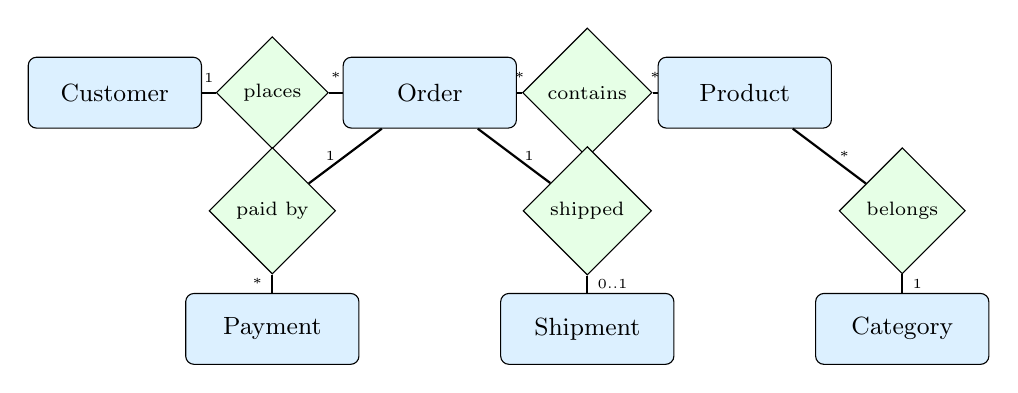
\begin{tikzpicture}[
    entity/.style={draw, fill=entitycolor, rounded corners=3pt, minimum width=2.2cm, minimum height=0.9cm, font=\small},
    relationship/.style={draw, diamond, fill=relationcolor, minimum width=1.4cm, minimum height=0.9cm, font=\scriptsize},
]
    % Entities
    \node[entity] (customer) at (0, 3) {Customer};
    \node[entity] (order) at (4, 3) {Order};
    \node[entity] (product) at (8, 3) {Product};
    \node[entity] (payment) at (2, 0) {Payment};
    \node[entity] (shipment) at (6, 0) {Shipment};
    \node[entity] (category) at (10, 0) {Category};
    
    % Relationships
    \node[relationship] (places) at (2, 3) {places};
    \node[relationship] (contains) at (6, 3) {contains};
    \node[relationship] (paidby) at (2, 1.5) {paid by};
    \node[relationship] (shippedvia) at (6, 1.5) {shipped};
    \node[relationship] (belongsto) at (10, 1.5) {belongs};
    
    % Connections with cardinality
    \draw[thick] (customer) -- (places) node[midway, above, font=\tiny] {1};
    \draw[thick] (places) -- (order) node[midway, above, font=\tiny] {*};
    \draw[thick] (order) -- (contains) node[midway, above, font=\tiny] {*};
    \draw[thick] (contains) -- (product) node[midway, above, font=\tiny] {*};
    \draw[thick] (order) -- (paidby) node[midway, left, font=\tiny] {1};
    \draw[thick] (paidby) -- (payment) node[midway, left, font=\tiny] {*};
    \draw[thick] (order) -- (shippedvia) node[midway, right, font=\tiny] {1};
    \draw[thick] (shippedvia) -- (shipment) node[midway, right, font=\tiny] {0..1};
    \draw[thick] (product) -- (belongsto) node[midway, right, font=\tiny] {*};
    \draw[thick] (belongsto) -- (category) node[midway, right, font=\tiny] {1};
    
\end{tikzpicture}
\caption{E-Commerce Conceptual Data Model}
\end{figure}

\textbf{Description:} This conceptual model shows the core business entities for an e-commerce system. Customers place Orders, which contain Products. Orders are paid by Payments and shipped via Shipments. Products belong to Categories. This high-level view communicates business concepts without implementation details.

\subsection{Example 2: Logical Data Model (Crow's Foot)}

\begin{figure}[H]
\centering
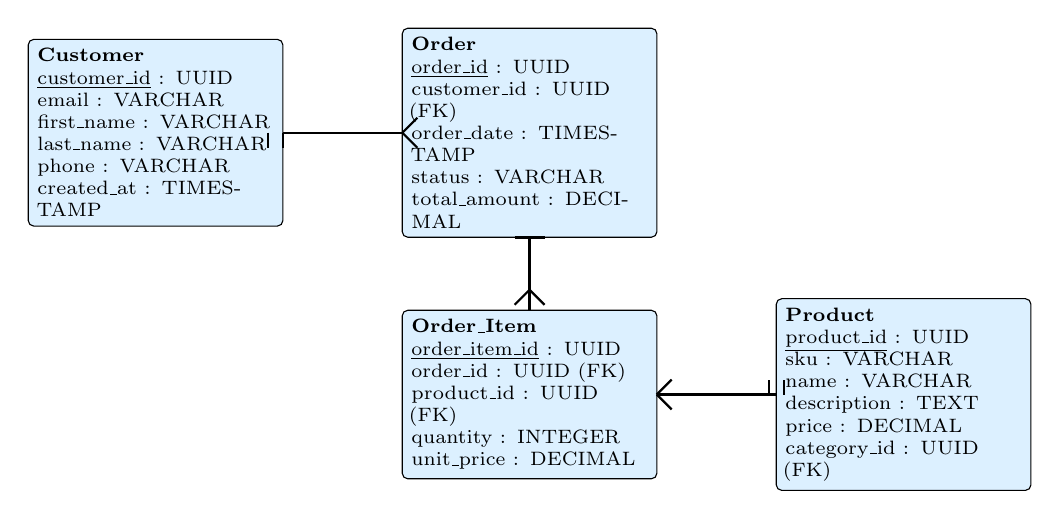
\begin{tikzpicture}[
    entity/.style={draw, fill=entitycolor, rounded corners=2pt, minimum width=3.2cm, text width=3cm, align=left, font=\scriptsize},
    scale=0.95
]
    % Customer Entity
    \node[entity] (customer) at (0, 3.5) {
        \textbf{Customer} \\
        \underline{customer\_id} : UUID \\
        email : VARCHAR \\
        first\_name : VARCHAR \\
        last\_name : VARCHAR \\
        phone : VARCHAR \\
        created\_at : TIMESTAMP
    };
    
    % Order Entity
    \node[entity] (order) at (5, 3.5) {
        \textbf{Order} \\
        \underline{order\_id} : UUID \\
        customer\_id : UUID (FK) \\
        order\_date : TIMESTAMP \\
        status : VARCHAR \\
        total\_amount : DECIMAL
    };
    
    % Order Item Entity
    \node[entity] (orderitem) at (5, 0) {
        \textbf{Order\_Item} \\
        \underline{order\_item\_id} : UUID \\
        order\_id : UUID (FK) \\
        product\_id : UUID (FK) \\
        quantity : INTEGER \\
        unit\_price : DECIMAL
    };
    
    % Product Entity
    \node[entity] (product) at (10, 0) {
        \textbf{Product} \\
        \underline{product\_id} : UUID \\
        sku : VARCHAR \\
        name : VARCHAR \\
        description : TEXT \\
        price : DECIMAL \\
        category\_id : UUID (FK)
    };
    
    % Relationships with Crow's Foot notation
    % Customer to Order (1 to many)
    \draw[thick] (customer.east) -- (order.west);
    \draw[thick] (1.7, 3.5) -- (1.7, 3.3);
    \draw[thick] (1.5, 3.5) -- (1.5, 3.3);
    \draw[thick] (3.3, 3.5) -- (3.5, 3.7);
    \draw[thick] (3.3, 3.5) -- (3.5, 3.3);
    
    % Order to Order_Item (1 to many)
    \draw[thick] (order.south) -- (orderitem.north);
    \draw[thick] (5, 2.1) -- (4.8, 2.1);
    \draw[thick] (5, 2.1) -- (5.2, 2.1);
    \draw[thick] (5, 1.4) -- (4.8, 1.2);
    \draw[thick] (5, 1.4) -- (5.2, 1.2);
    
    % Order_Item to Product (many to 1)
    \draw[thick] (orderitem.east) -- (product.west);
    \draw[thick] (6.7, 0) -- (6.9, 0.2);
    \draw[thick] (6.7, 0) -- (6.9, -0.2);
    \draw[thick] (8.2, 0) -- (8.2, 0.2);
    \draw[thick] (8.4, 0) -- (8.4, 0.2);
    
\end{tikzpicture}
\caption{E-Commerce Logical Data Model (Partial)}
\end{figure}

\textbf{Description:} This logical model shows detailed entity definitions with attributes, data types, and keys. The Crow's Foot notation indicates cardinality: Customer has many Orders, Order has many Order\_Items, and Order\_Item references one Product. This model is implementation-independent but fully specified.

\subsection{Example 3: Data Flow Diagram}

\begin{figure}[H]
\centering
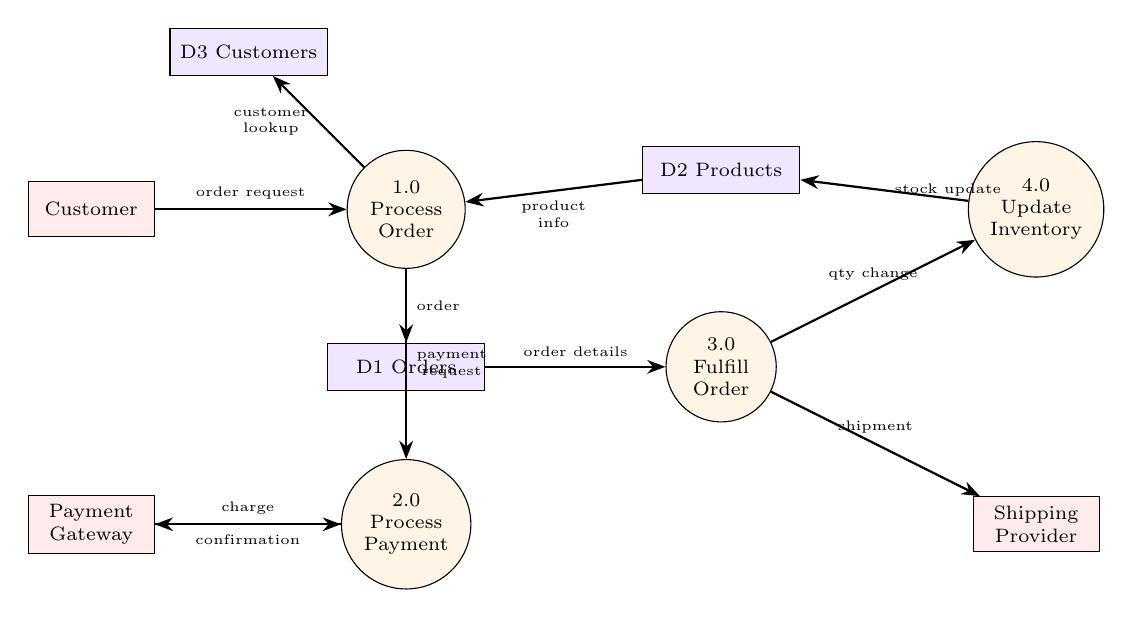
\begin{tikzpicture}[
    process/.style={draw, circle, fill=processcolor, minimum size=1.4cm, font=\scriptsize, align=center},
    store/.style={draw, fill=storecolor, minimum width=2cm, minimum height=0.6cm, font=\scriptsize},
    external/.style={draw, fill=flowcolor, minimum width=1.6cm, minimum height=0.7cm, font=\scriptsize},
    flow/.style={-{Stealth}, thick}
]
    % External Entities
    \node[external] (customer) at (-4, 2) {Customer};
    \node[external] (payment) at (-4, -2) {Payment\\Gateway};
    \node[external] (shipping) at (8, -2) {Shipping\\Provider};
    
    % Processes
    \node[process] (orderproc) at (0, 2) {1.0\\Process\\Order};
    \node[process] (payproc) at (0, -2) {2.0\\Process\\Payment};
    \node[process] (shipproc) at (4, 0) {3.0\\Fulfill\\Order};
    \node[process] (inventory) at (8, 2) {4.0\\Update\\Inventory};
    
    % Data Stores
    \node[store] (orderdb) at (0, 0) {D1 Orders};
    \node[store] (productdb) at (4, 2.5) {D2 Products};
    \node[store] (custdb) at (-2, 4) {D3 Customers};
    
    % Flows
    \draw[flow] (customer) -- (orderproc) node[midway, above, font=\tiny] {order request};
    \draw[flow] (orderproc) -- (orderdb) node[midway, right, font=\tiny] {order};
    \draw[flow] (orderproc) -- (payproc) node[midway, right, font=\tiny] {payment\\request};
    \draw[flow] (payproc) -- (payment) node[midway, above, font=\tiny] {charge};
    \draw[flow] (payment) -- (payproc) node[midway, below, font=\tiny] {confirmation};
    \draw[flow] (orderdb) -- (shipproc) node[midway, above, font=\tiny] {order details};
    \draw[flow] (shipproc) -- (shipping) node[midway, above, font=\tiny] {shipment};
    \draw[flow] (shipproc) -- (inventory) node[midway, above, font=\tiny] {qty change};
    \draw[flow] (inventory) -- (productdb) node[midway, right, font=\tiny] {stock update};
    \draw[flow] (orderproc) -- (custdb) node[midway, left, font=\tiny] {customer\\lookup};
    \draw[flow] (productdb) -- (orderproc) node[midway, below, font=\tiny] {product\\info};
    
\end{tikzpicture}
\caption{Order Processing Data Flow Diagram}
\end{figure}

\textbf{Description:} This DFD shows data movement through an order processing system. External entities (Customer, Payment Gateway, Shipping Provider) interact with processes. Data stores (Orders, Products, Customers) persist data. Arrows show data flows with labels indicating the data items transferred.

\subsection{Example 4: Data Classification Schema}

\begin{table}[H]
\centering
\caption{Data Classification Matrix}
\small
\begin{tabular}{@{}L{2cm}L{2.5cm}L{4cm}L{4.5cm}@{}}
\toprule
\textbf{Level} & \textbf{Examples} & \textbf{Handling Requirements} & \textbf{Access} \\
\midrule
\cellcolor{green!20}\textbf{Public} & Product catalog, Public content & No restrictions & Anyone \\
\addlinespace
\cellcolor{yellow!20}\textbf{Internal} & Employee directory, Internal docs & Internal network only, no external sharing & Employees \\
\addlinespace
\cellcolor{orange!20}\textbf{Confidential} & Customer PII, Financial data & Encryption required, audit logging, need-to-know & Authorized roles \\
\addlinespace
\cellcolor{red!20}\textbf{Restricted} & Payment cards, Health records, Auth credentials & Strong encryption, MFA, strict audit, minimal retention & Named individuals \\
\bottomrule
\end{tabular}
\end{table}

\textbf{Description:} This classification schema defines four sensitivity levels with corresponding handling requirements and access restrictions. Each data element must be classified, and the classification determines applicable security controls.

% =============================================================================
% SECTION: NOTES
% =============================================================================
\section{Notes}

\subsection{Privacy and Compliance Considerations}

\begin{privacybox}[Privacy by Design Principles]
When developing information architecture, incorporate privacy from the start:

\begin{enumerate}[nosep]
    \item \textbf{Data Minimization:} Collect only necessary data
    \item \textbf{Purpose Limitation:} Use data only for stated purposes
    \item \textbf{Storage Limitation:} Retain only as long as needed
    \item \textbf{Consent Management:} Track and honor consent preferences
    \item \textbf{Right to Access:} Enable data subject access requests
    \item \textbf{Right to Erasure:} Support data deletion requests
    \item \textbf{Data Portability:} Enable data export in standard formats
\end{enumerate}
\end{privacybox}

\subsection{Versioning Considerations}

Data models evolve over time and require careful version management:

\begin{itemize}
    \item Maintain schema version history with change documentation
    \item Use database migration tools (Flyway, Liquibase, Alembic)
    \item Plan backward compatibility for schema changes
    \item Document breaking vs. non-breaking changes
    \item Coordinate schema changes across dependent systems
    \item Implement schema registry for event-driven systems
\end{itemize}

\subsection{Tooling Recommendations}

\begin{table}[H]
\centering
\caption{Recommended Tools by Use Case}
\small
\begin{tabular}{@{}L{3.5cm}L{10cm}@{}}
\toprule
\textbf{Use Case} & \textbf{Recommended Tools} \\
\midrule
Data Modeling & ERwin, PowerDesigner, Lucidchart, dbdiagram.io, SqlDBM \\
Data Catalog & Collibra, Alation, DataHub, Apache Atlas, AWS Glue \\
Data Quality & Great Expectations, dbt tests, Soda, Monte Carlo \\
Data Lineage & Collibra, Atlan, OpenLineage, dbt \\
Schema Migration & Flyway, Liquibase, Alembic, Atlas \\
Data Masking & Delphix, Informatica, AWS DMS \\
\bottomrule
\end{tabular}
\end{table}

\subsection{Common Pitfalls}

\begin{warningbox}[Common Mistakes to Avoid]
\begin{enumerate}[nosep]
    \item \textbf{Skipping Conceptual Model:} Jumping to physical design without business alignment
    \item \textbf{Over-Normalization:} Creating performance problems with excessive joins
    \item \textbf{Under-Normalization:} Creating data anomalies with insufficient normalization
    \item \textbf{Ignoring Data Quality:} Assuming data will be clean without validation
    \item \textbf{Missing Audit Trail:} Not tracking who changed what and when
    \item \textbf{Hardcoded Values:} Embedding reference data in application code
    \item \textbf{Unclear Ownership:} No defined responsibility for data domains
    \item \textbf{Security Afterthought:} Adding data protection after design is complete
\end{enumerate}
\end{warningbox}

% =============================================================================
% SECTION: SOURCES
% =============================================================================
\section{Sources}

\subsection{Primary References}

\begin{enumerate}
    \item Clements, P., Bachmann, F., Bass, L., Garlan, D., Ivers, J., Little, R., Merson, P., Nord, R., \& Stafford, J. (2010). \textit{Documenting Software Architectures: Views and Beyond} (2nd ed.). Addison-Wesley Professional.
    
    \item ISO/IEC/IEEE 42010:2011. \textit{Systems and software engineering --- Architecture description}. International Organization for Standardization.
    
    \item Hoberman, S. (2009). \textit{Data Modeling Made Simple} (2nd ed.). Technics Publications.
    
    \item Kimball, R. \& Ross, M. (2013). \textit{The Data Warehouse Toolkit} (3rd ed.). Wiley.
    
    \item DAMA International. (2017). \textit{DAMA-DMBOK: Data Management Body of Knowledge} (2nd ed.). Technics Publications.
\end{enumerate}

\subsection{Supplementary References}

\begin{enumerate}[resume]
    \item Fowler, M. (2002). \textit{Patterns of Enterprise Application Architecture}. Addison-Wesley Professional.
    
    \item Evans, E. (2003). \textit{Domain-Driven Design}. Addison-Wesley Professional.
    
    \item Kleppmann, M. (2017). \textit{Designing Data-Intensive Applications}. O'Reilly Media.
    
    \item Linstedt, D. \& Olschimke, M. (2015). \textit{Building a Scalable Data Warehouse with Data Vault 2.0}. Morgan Kaufmann.
    
    \item Reis, J. \& Housley, M. (2022). \textit{Fundamentals of Data Engineering}. O'Reilly Media.
\end{enumerate}

\subsection{Online Resources}

\begin{itemize}
    \item DAMA International: \url{https://www.dama.org/}
    \item Data Modeling Zone: \url{https://www.datamodelzone.com/}
    \item dbdiagram.io: \url{https://dbdiagram.io/}
    \item Great Expectations: \url{https://greatexpectations.io/}
    \item dbt Documentation: \url{https://docs.getdbt.com/}
\end{itemize}

% =============================================================================
% APPENDIX
% =============================================================================
\appendix

\section{Information View Checklist}

Use this checklist to verify completeness of information architecture documentation:

\begin{table}[H]
\centering
\small
\begin{tabular}{@{}L{10cm}C{2cm}@{}}
\toprule
\textbf{Item} & \textbf{Complete?} \\
\midrule
\multicolumn{2}{l}{\textbf{Data Modeling}} \\
\quad Conceptual model with business stakeholder approval & $\square$ \\
\quad Logical model with full attribute specifications & $\square$ \\
\quad Physical model with technology-specific details & $\square$ \\
\quad Entity relationships with cardinality defined & $\square$ \\
\quad Constraints documented and justified & $\square$ \\
\midrule
\multicolumn{2}{l}{\textbf{Data Flow and Integration}} \\
\quad Data flows identified and documented & $\square$ \\
\quad Integration patterns specified & $\square$ \\
\quad Transformations documented & $\square$ \\
\quad Error handling defined & $\square$ \\
\midrule
\multicolumn{2}{l}{\textbf{Data Governance}} \\
\quad Data classification applied to all entities & $\square$ \\
\quad Data quality rules defined & $\square$ \\
\quad Retention policies established & $\square$ \\
\quad Data ownership assigned & $\square$ \\
\quad Stewardship responsibilities defined & $\square$ \\
\midrule
\multicolumn{2}{l}{\textbf{Security and Privacy}} \\
\quad Sensitive data identified and classified & $\square$ \\
\quad Access control requirements specified & $\square$ \\
\quad Encryption requirements documented & $\square$ \\
\quad Privacy requirements addressed (GDPR, CCPA) & $\square$ \\
\quad Audit requirements defined & $\square$ \\
\midrule
\multicolumn{2}{l}{\textbf{Validation}} \\
\quad Correspondence with other views verified & $\square$ \\
\quad Business stakeholder review completed & $\square$ \\
\quad Technical review completed & $\square$ \\
\quad Compliance review completed & $\square$ \\
\bottomrule
\end{tabular}
\end{table}

\section{Glossary}

\begin{description}[style=nextline, leftmargin=3cm, labelwidth=2.8cm]
    \item[Attribute] A property of an entity that captures a specific piece of information.
    
    \item[Cardinality] The number of instances of one entity that can be associated with instances of another entity.
    
    \item[CDC] Change Data Capture; a technique for identifying and capturing changes to data.
    
    \item[Conceptual Model] A high-level data model representing business entities and relationships.
    
    \item[Data Catalog] A metadata repository that provides information about data assets.
    
    \item[Data Classification] Categorization of data based on sensitivity and handling requirements.
    
    \item[Data Flow] Movement of data between components, systems, or processes.
    
    \item[Data Lineage] The tracking of data's origin, movement, and transformation over time.
    
    \item[Data Quality] The degree to which data meets requirements for accuracy, completeness, and consistency.
    
    \item[Data Steward] An individual responsible for data quality and governance within a domain.
    
    \item[Entity] A distinguishable object or concept about which data is captured.
    
    \item[ETL] Extract, Transform, Load; a data integration pattern.
    
    \item[Foreign Key] An attribute that references a primary key in another entity.
    
    \item[Logical Model] A detailed data model independent of physical implementation.
    
    \item[Master Data] Core business entities shared across the organization.
    
    \item[Normalization] The process of organizing data to reduce redundancy and improve integrity.
    
    \item[Physical Model] An implementation-specific data model for a particular technology.
    
    \item[PII] Personally Identifiable Information; data that can identify an individual.
    
    \item[Primary Key] An attribute or set of attributes that uniquely identifies an entity instance.
    
    \item[Relationship] An association between two or more entities.
    
    \item[Retention Policy] Rules governing how long data is kept before archival or deletion.
\end{description}

\section{Entity Specification Template}

\begin{lstlisting}[caption={Complete Entity Specification Template}, language={}]
================================================================================
ENTITY SPECIFICATION
================================================================================

1. IDENTIFICATION
-----------------
Entity ID:          [ENT-XXX]
Name:               [Entity Name]
Domain:             [Business Domain]
Version:            [X.Y]
Status:             [Draft | Review | Approved | Deprecated]
Owner:              [Data Owner]
Steward:            [Data Steward]
Last Updated:       [Date]

2. BUSINESS DESCRIPTION
-----------------------
Definition:
  [Clear business definition of what this entity represents]

Business Rules:
  - [Business rule 1]
  - [Business rule 2]

Usage Context:
  [How and where this entity is used in business processes]

3. ATTRIBUTES
-------------
+---------------+----------+------+-----+---------+-------+-------------------+
| Name          | Type     | Null | Key | Default | Class | Description       |
+---------------+----------+------+-----+---------+-------+-------------------+
| [name]        | [type]   | Y/N  | PK  | [val]   | [C/I] | [description]     |
| [name]        | [type]   | Y/N  | FK  | [val]   | [C/I] | [description]     |
| [name]        | [type]   | Y/N  |     | [val]   | [C/I] | [description]     |
+---------------+----------+------+-----+---------+-------+-------------------+

Key: PK=Primary Key, FK=Foreign Key, UK=Unique Key, AK=Alternate Key
Class: C=Confidential, I=Internal, P=Public, R=Restricted

4. RELATIONSHIPS
----------------
+------------------+----------------+-------------+---------------------------+
| Relationship     | Related Entity | Cardinality | Description               |
+------------------+----------------+-------------+---------------------------+
| [verb phrase]    | [Entity]       | [1:N]       | [description]             |
+------------------+----------------+-------------+---------------------------+

5. CONSTRAINTS
--------------
+------------------+----------+------------------------------------------+
| Constraint Name  | Type     | Definition                               |
+------------------+----------+------------------------------------------+
| [name]           | [type]   | [constraint definition]                  |
+------------------+----------+------------------------------------------+

Types: PK, FK, UK, CHECK, NOT NULL, DEFAULT

6. DATA CLASSIFICATION
----------------------
Sensitivity Level:  [Public | Internal | Confidential | Restricted]
Contains PII:       [Yes | No]
PII Elements:       [List of PII attributes if applicable]
Regulations:        [GDPR | CCPA | HIPAA | PCI-DSS | SOX | etc.]
Encryption:         [At Rest | In Transit | Both | None]

7. DATA QUALITY RULES
---------------------
+----------+-------------+---------------------+----------+------------------+
| Rule ID  | Attribute   | Rule                | Severity | Action           |
+----------+-------------+---------------------+----------+------------------+
| [DQ-XXX] | [attribute] | [rule description]  | [level]  | [action]         |
+----------+-------------+---------------------+----------+------------------+

Severity: Critical, Major, Minor, Warning
Action: Reject, Flag, Correct, Notify

8. LIFECYCLE
------------
Creation:           [How data is created]
Retention Period:   [Duration]
Archival Policy:    [Policy description]
Deletion Policy:    [Policy description]
Legal Hold:         [Applicable | Not Applicable]

9. PHYSICAL IMPLEMENTATION
--------------------------
Database:           [Database name]
Schema:             [Schema name]
Table:              [Table name]
Partitioning:       [Strategy if applicable]
Indexes:            [Key indexes]

10. LINEAGE
-----------
Source Systems:     [List of source systems]
Target Systems:     [List of consuming systems]
Transformations:    [Key transformations applied]

11. CHANGE HISTORY
------------------
+------------+---------+---------------+-----------------------------------+
| Date       | Version | Author        | Change Description                |
+------------+---------+---------------+-----------------------------------+
| [date]     | [X.Y]   | [name]        | [description]                     |
+------------+---------+---------------+-----------------------------------+

================================================================================
\end{lstlisting}

% =============================================================================
% END DOCUMENT
% =============================================================================

\end{document}
